\documentclass{beamer}

% for themes, etc.
\mode<presentation>{ 
\usetheme{Rochester} 
}

\usepackage{cancel}
\usepackage{array}
\usepackage{graphicx}
\usepackage{tikz}
\usetikzlibrary{shapes, arrows, positioning}

\title[]{A Surrogate Approach Towards Validation and Uncertainty Quantification of Multiphysics Reactor Simulation Codes}
\subtitle[]{Thesis Prospectus}
\author[]{Artem Yankov}
\institute[]{University of Michigan}
\date{April 17, 2014}

% have this if you'd like a recurring outline
\AtBeginSection[]  % "Beamer, do the following at the start of every section"
{
\begin{frame}<beamer> 
\frametitle{Outline} % make a frame titled "Outline"
\tableofcontents[currentsection]  % show TOC and highlight current section
\end{frame}
}

\begin{document}

% this prints title, author etc. info from above
\begin{frame}
\titlepage
\end{frame}

% MOTIVATION
\section{Motivation}

%%%%%%%%%%%%%%%%%%%%%%%%%%%%%%%%%%%%%%%%%%%%%%%%%%%%%%%%%%%%%%%%%%%%%%%%%%%%%%%%%%%%%%%%
\begin{frame}
\frametitle{Background}

\begin{itemize}
  \item Physical phenomena is studied by conducting experiments. 
  \item Any data collected represents instances of underlying stochastic processes.  
  \item We build predictive computer models in an attempt to reproduce such observed physical phenomena.
  \item To accurately capture stochastic element of experiments, computer models should be probabilistic.  
  \item In other words, inputs to computer models have uncertainties associated with them that are propagated to any outputs of interest.
  \item Running computer simulations should be like conducting physical experiments. Computer experiments.      
\end{itemize}

\end{frame}
%%%%%%%%%%%%%%%%%%%%%%%%%%%%%%%%%%%%%%%%%%%%%%%%%%%%%%%%%%%%%%%%%%%%%%%%%%%%%%%%%%%%%%%%
\begin{frame}
\frametitle{Why Surrogates?}

\begin{itemize}
  \item We run computer simulations to meet design objectives under certain constraints. 
  \item Involves numerical optimization, calibration, and performing what-if analyses.
  \item Also, we're interested in determining which of our design variables have the greatest effects on simulation outcomes. 
  \item Thousands of simulations required to make this possible but...  
  \item Computer simulations that model real phenomenon like nuclear reactors often take $\mathcal{O}(\mbox{hours})$ or $\mathcal{O}(\mbox{days})$ to complete.
  \item Building a surrogate model for your expensive computer simulations can make everything listed above possible.   
\end{itemize}

\end{frame}
%%%%%%%%%%%%%%%%%%%%%%%%%%%%%%%%%%%%%%%%%%%%%%%%%%%%%%%%%%%%%%%%%%%%%%%%%%%%%%%%%%%%%%%%
\begin{frame}
\frametitle{What is a Surrogate Model?}

\begin{itemize}
  \item A model for the outcomes of (likely) expensive computer simulations that can be rapidly evaluated while simultaneously preserving the predictive capabilities of the original simulations.
  \item Want to intelligently choose subspace $\lbrace x_1, x_2, ..., x_N\rbrace \subset \mathbf{X}$ to sample expensive computer code to get $\lbrace y_1, y_2, ..., y_N\rbrace \subset \mathbf{Y}$.
  \item Learn fast mapping that approximates $\mathbf{X}\rightarrow\mathbf{Y}$.   
\end{itemize}

\begin{figure}
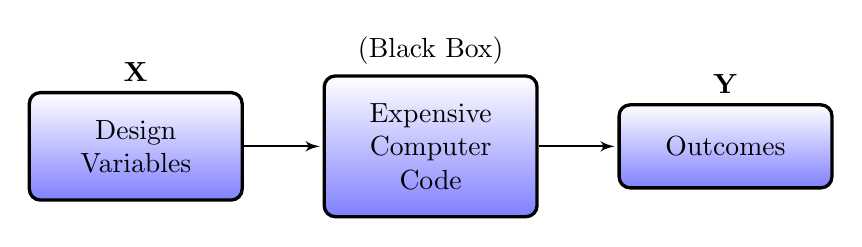
\begin{tikzpicture}[node distance=1cm, auto]  
\tikzset{
    mynode/.style={rectangle,rounded corners,draw=black, top color=white, bottom color=blue!50,very thick, inner sep=1em, minimum size=3em, text centered},
    myarrow/.style={->, >=latex', shorten >=1pt, thick},
    mylabel/.style={text width=7em, text centered} 
}  
\node[mynode, text width=2cm, label=$\mathbf{X}$] (design_vars) {Design Variables};  
\node[mynode, right= of design_vars, text width=2cm, label=(Black Box)] (computer_code) {Expensive Computer Code};
\node[mynode, right= of computer_code, text width=2cm, label=$\mathbf{Y}$] (outcomes) {Outcomes};
\draw[myarrow] (design_vars) edge node {} (computer_code);
\draw[myarrow] (computer_code) edge node {} (outcomes);
\end{tikzpicture}  
\end{figure}

\end{frame}

% PROPOSED APPLICATION
\subsection{Proposed Application}
%%%%%%%%%%%%%%%%%%%%%%%%%%%%%%%%%%%%%%%%%%%%%%%%%%%%%%%%%%%%%%%%%%%%%%%%%%%%%%%%%%%%%%%%
\begin{frame}
\frametitle{Proposed Application to Fuel Performance Modeling}

\begin{itemize}
  \item Fission Gas Release (FGR) refers to the phenomenon where Xenon and Krypton gases formed in UO$_2$ fuel rods are released into the rod filling gas.
  \item Causes pressure build-up and thermal conductivity degradation in the rod filling gas, potentially jeopardizing the safety of the reactor.
  \item Fission gas atoms generated in the fuel grains diffuse towards the grain boundaries. 
  \item Majority of the gas diffuses into grain-face gas bubbles, giving rise to grain-face swelling.
  \item Bubble growth brings about bubble coalescence and interconnection, eventually leading to the formation of a tunnel network through which the fission gas is released.       
\end{itemize}

\end{frame}   
%%%%%%%%%%%%%%%%%%%%%%%%%%%%%%%%%%%%%%%%%%%%%%%%%%%%%%%%%%%%%%%%%%%%%%%%%%%%%%%%%%%%%%%%
\begin{frame}
\frametitle{SIFGRS FGR Model}

\begin{itemize}
  \item Simple Integrated Fission Gas Release and Swelling (SIFGRS)
  \item Incorporates gas diffusion and precipitation in grains, growth and coalescence of gas bubbles at grain faces, thermal, athermal, steady-state, and transient gas release. 
  \item Through a direct description of the grain face gas bubble development, the fission gas swelling and release are calculated as coupled processes.
  \item Parameterized by, among others, linear heat rate, gas diffusion coefficient, surface tension of grain face bubbles, hydrostatic pressure, fuel grain radius, fuel porosity, and grain boundary sweeping. 
\end{itemize}

\end{frame}
%%%%%%%%%%%%%%%%%%%%%%%%%%%%%%%%%%%%%%%%%%%%%%%%%%%%%%%%%%%%%%%%%%%%%%%%%%%%%%%%%%%%%%%%
\begin{frame}
\frametitle{Ris\o~AN3 Experiment}

\begin{itemize}
  \item Validation case for fuel performance modeling in the Fumex-II database.
  \item Experiment consists of a base irradiation of four reactor cycles in the Biblis A pressurized water reactor.
  \item After the base irradiation period, a fuel rod is extracted and refabricated to a shorter length before undergoing a power ramp.
  \item Refabricated fuel rod is outfitted with various instrumentation such that fuel centerline temperature, FGR and rod internal pressure measurements can be obtained.    
\end{itemize}

\end{frame}
%%%%%%%%%%%%%%%%%%%%%%%%%%%%%%%%%%%%%%%%%%%%%%%%%%%%%%%%%%%%%%%%%%%%%%%%%%%%%%%%%%%%%%%%
\begin{frame}
\frametitle{Ris\o~AN3 Experiment Irradiation Profiles}

\begin{columns}
 \begin{column}{0.5\textwidth}
  \centering
  Base Irradiation History
  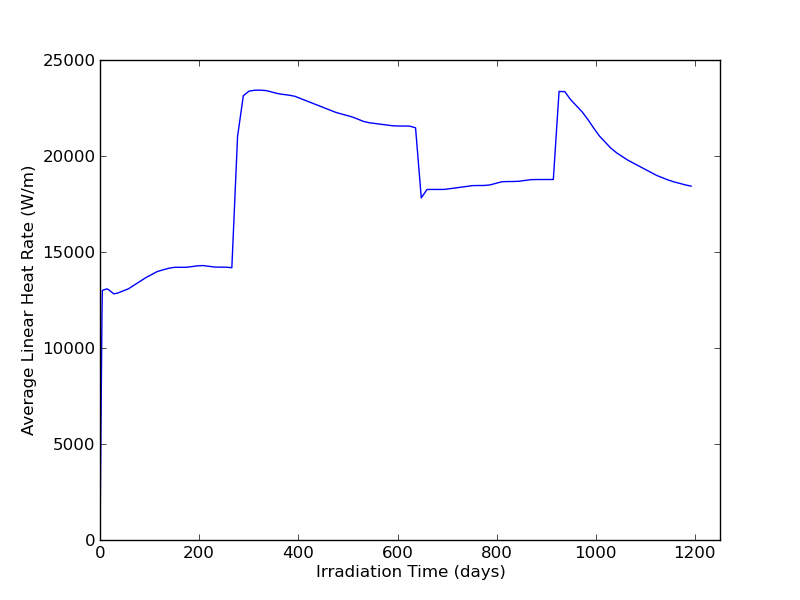
\includegraphics[width=1.\textwidth]{./base_irrad.png}
 \end{column}
 \begin{column}{0.5\textwidth}
  \centering
  Power Ramp Experiment
  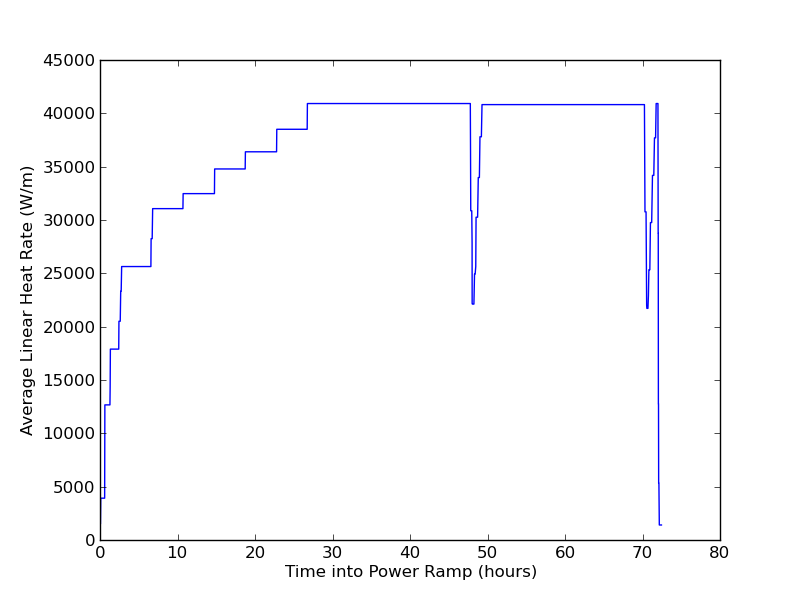
\includegraphics[width=1.\textwidth]{./power_ramp.png}
 \end{column}
\end{columns}

\end{frame}
%%%%%%%%%%%%%%%%%%%%%%%%%%%%%%%%%%%%%%%%%%%%%%%%%%%%%%%%%%%%%%%%%%%%%%%%%%%%%%%%%%%%%%%%
\begin{frame}
\frametitle{Modeling Ris\o~AN3 Experiment with BISON}

\begin{itemize}
  \item BISON is a finite-element fuel performance modeling code that utilizes the SIFGRS model.
  \item SIFGRS parameters are quite generic and uncertain. 
\end{itemize}

\begin{columns}
 \begin{column}{0.5\textwidth}
  \centering
  Fission Gas Release
  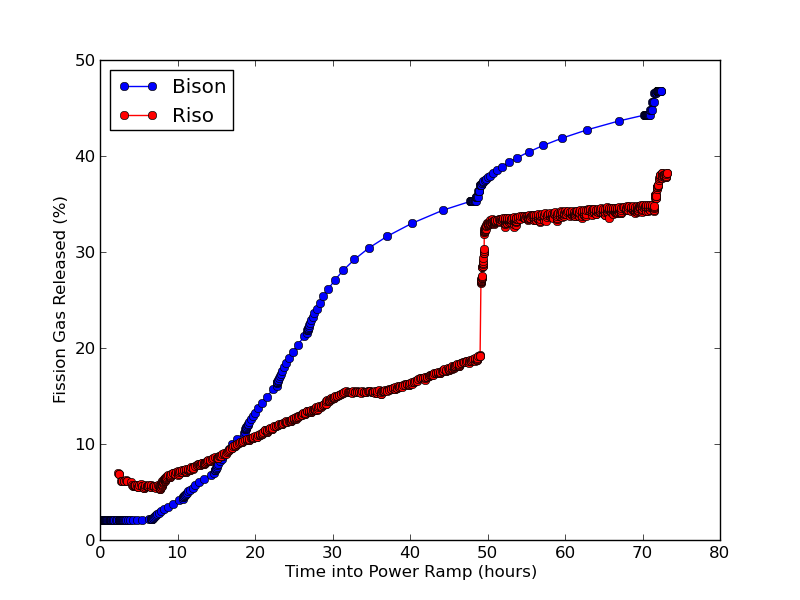
\includegraphics[width=1.\textwidth]{./fgr_comparison.png}
 \end{column}
 \begin{column}{0.5\textwidth}
  \centering
  Fuel Centerline Temperature
  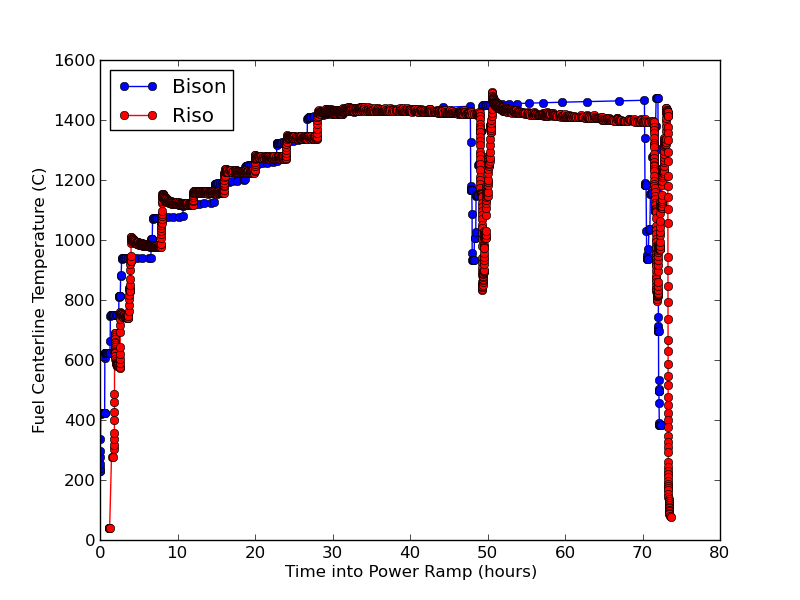
\includegraphics[width=1.\textwidth]{./tc_temp_comparison.png}
 \end{column}
\end{columns}

\end{frame}
%%%%%%%%%%%%%%%%%%%%%%%%%%%%%%%%%%%%%%%%%%%%%%%%%%%%%%%%%%%%%%%%%%%%%%%%%%%%%%%%%%%%%%%%
\begin{frame}
\frametitle{Modeling Ris\o~AN3 Experiment with BISON/MPACT}

\begin{itemize}
  \item No sense in comparing the output of a computer simulation to
experimental data unless the computer simulation is of high fidelity and capable
of reproducing the pertinent physics.
  \item MPACT is a neutronics code that provides detailed intrapin and azimuthally dependent
neutronics data in the fuel elements. 
  \item The two-way coupling scheme provided by BISON and MPACT provides the most accurate fuel performance modeling available for a nuclear reactor.
  \item Expensive! 
\end{itemize}

\end{frame}
%%%%%%%%%%%%%%%%%%%%%%%%%%%%%%%%%%%%%%%%%%%%%%%%%%%%%%%%%%%%%%%%%%%%%%%%%%%%%%%%%%%%%%%%
\begin{frame}
\frametitle{Modeling Ris\o~AN3 Experiment with BISON/MPACT}

\begin{itemize}
  \item BISON predictions of FGR and temperature fields stand to be improved by calibrating FGR parameters to experimental data.
  \item Calibration studies require $\mathcal{O}(10^3)$ function evaluations, which in this case are the coupled BISON/MPACT computer codes.
  \item Each simulation of the Ris\o~AN3 experiment will take a few hours.
  \item It's necessary to construct a surrogate for the calibration study!   
\end{itemize}

\end{frame}
%%%%%%%%%%%%%%%%%%%%%%%%%%%%%%%%%%%%%%%%%%%%%%%%%%%%%%%%%%%%%%%%%%%%%%%%%%%%%%%%%%%%%%%%

% SURROGATE CONSTRUCTION
\section{Surrogate Models}

% OVERVIEW
\subsection{Overview}
%%%%%%%%%%%%%%%%%%%%%%%%%%%%%%%%%%%%%%%%%%%%%%%%%%%%%%%%%%%%%%%%%%%%%%%%%%%%%%%%%%%%%%%%
\begin{frame}
\frametitle{Classic Overview}

\begin{figure}
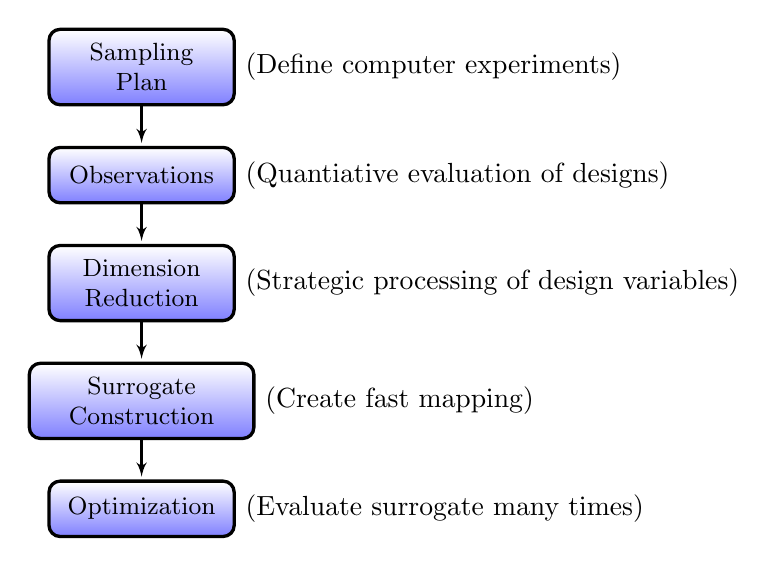
\begin{tikzpicture}[node distance=0.5cm, auto]  
\tikzset{
    mynode/.style={rectangle,rounded corners,draw=black, top color=white, bottom color=blue!50, very thick, inner sep=.5em, minimum size=2em, text centered, font=\small},
    myarrow/.style={->, >=latex', shorten >=1pt, thick}
}  
\node[mynode, text width=2cm, label=right:(Define computer experiments)](samp_plan) {Sampling Plan};
\node[mynode, below= of samp_plan, text width=2cm, label=right:(Quantiative evaluation of designs)](obs) {Observations};
\node[mynode, below= of obs, text width=2cm, label=right:(Strategic processing of design variables)](dim_red) {Dimension Reduction};
\node[mynode, below= of dim_red, text width=2.5cm, label=right:(Create fast mapping)](surr) {Surrogate Construction};
\node[mynode, below= of surr, text width=2cm, label=right:(Evaluate surrogate many times)](opt) {Optimization};
\draw[myarrow] (samp_plan) edge node {} (obs);
\draw[myarrow] (obs) edge node {} (dim_red);
\draw[myarrow] (dim_red) edge node {} (surr);
\draw[myarrow] (surr) edge node {} (opt);
\end{tikzpicture}  
\end{figure}

\end{frame}
%%%%%%%%%%%%%%%%%%%%%%%%%%%%%%%%%%%%%%%%%%%%%%%%%%%%%%%%%%%%%%%%%%%%%%%%%%%%%%%%%%%%%%%%
\begin{frame}
\frametitle{Kriging vs. anchored-ANOVA Collocation}

\begin{columns}
 \begin{column}{0.5\textwidth}
  Kriging
  \begin{itemize}
    \item Dimension reduction processed separately
    \item Sampling points random
    \item User determines how many points to use for sampling plan
    \item Interpolation by covariance basis functions
    \item More statistical approach
  \end{itemize}
 \end{column}
 \begin{column}{0.5\textwidth}
 anchored-ANOVA Collocation
  \begin{itemize}
    \item Dimension reduction inherent
    \item Sampling done on structured grid
    \item Sampling plan size dependent on number of design variables
    \item Polynomial interpolation
    \item More deterministic approach
  \end{itemize}
 \end{column}
\end{columns}

\end{frame}
%%%%%%%%%%%%%%%%%%%%%%%%%%%%%%%%%%%%%%%%%%%%%%%%%%%%%%%%%%%%%%%%%%%%%%%%%%%%%%%%%%%%%%%%
\subsection{Kriging}

%%%%%%%%%%%%%%%%%%%%%%%%%%%%%%%%%%%%%%%%%%%%%%%%%%%%%%%%%%%%%%%%%%%%%%%%%%%%%%%%%%%%%%%%
\begin{frame}
\frametitle{Dimension Reduction for Kriging}

\begin{itemize}
  \item Kriging effective for $\mathcal{O}(10)$ design variables.
  \item For more design variables Kriging will defeat the purpose of having a surrogate in the first place.
  \item Fortunately, various engineering applications have shown that only a handful of design variables have non trivial impact on outputs of interest.
  \item How to identify the "important variables"?
  \item Morris' Algorithm.   
\end{itemize}

\end{frame}
%%%%%%%%%%%%%%%%%%%%%%%%%%%%%%%%%%%%%%%%%%%%%%%%%%%%%%%%%%%%%%%%%%%%%%%%%%%%%%%%%%%%%%%%
\begin{frame}
\frametitle{Morris' Algorithm}

\begin{itemize}
  \item Premise: If the output parameter does not change with respect to a design variable then the variable can safely be ignored.
  \item Elementary effect $d_i\left(\textbf{x}\right)$ of design variable $x_i$:
\begin{align*}
 d_i\left(\textbf{x}\right) = \frac{f\left(x_1,x_2,...,x_{i-1},x_i+\Delta,x_{i+1},....,x_k 									\right) - f\left(\textbf{x}\right)}{\Delta}      
\end{align*} 
  \item Choosing a set of $\textbf{x}$ carefully, it is possible to calculate an elementary effect for each of $k$ design variables using only $k+1$ function evaluations using the random orientation matrix $\textbf{B}^*$: 
\begin{align*}
 \textbf{B}^* = \left(\textbf{1}_{k+1,1}\textbf{x}^* + \frac{\Delta}{2}\left[
                 \left(2\textbf{B} - \textbf{1}_{k+1,k}\right)\textbf{D}^* + 
                  \textbf{1}_{k+1,k}\right]\right)\textbf{P}^*.
\end{align*}                
\end{itemize}

\end{frame}
%%%%%%%%%%%%%%%%%%%%%%%%%%%%%%%%%%%%%%%%%%%%%%%%%%%%%%%%%%%%%%%%%%%%%%%%%%%%%%%%%%%%%%%%
\begin{frame}
\frametitle{Morris' Algorithm}

\begin{itemize}
  \item $r$ random orientation matrices are created to obtain $r$ elementary effects for each design variable. 
  \item Plot mean and standard deviation of each variable's effects.
  \item Variables with negligible effect on function will cluster around origin. 
  \item Large fluctuations in standard deviation indicative of nonlinear and interactive effects.              
\end{itemize}

\centering
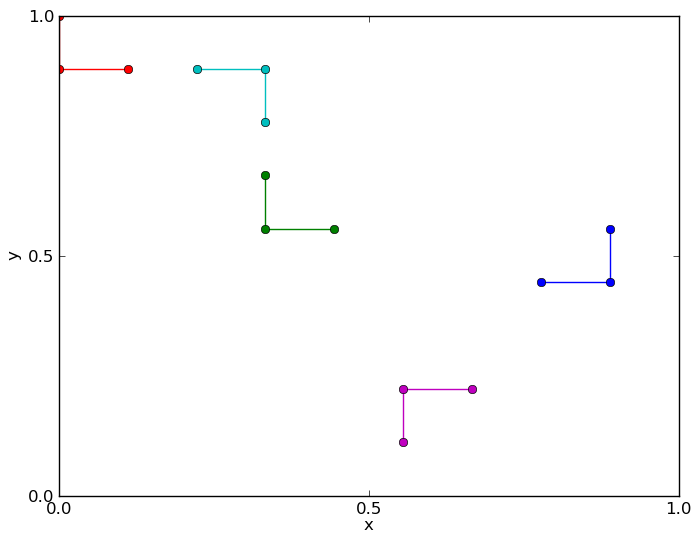
\includegraphics[width=0.50\textwidth]{./morris_alg.png}

\end{frame}
%%%%%%%%%%%%%%%%%%%%%%%%%%%%%%%%%%%%%%%%%%%%%%%%%%%%%%%%%%%%%%%%%%%%%%%%%%%%%%%%%%%%%%%%
\begin{frame}
\frametitle{Designing a Kriging Sampling Plan}

\begin{itemize}
  \item All surrogate models are built around a set of points at which the objective computer code is actually evaluated. 
  \item Intuitively, the surrogate accuracy is expected to decrease as one moves further away from such points. 
  \item Important to spread $N$ points as uniformly as possible across the design space.
  \item For Kriging, Latin Hypercube Sampling (LHS) is used to create a sampling plan.
  \item There is a notion of an optimized LHS sampling plan based on the maximin metric.   
\end{itemize}

\end{frame}
%%%%%%%%%%%%%%%%%%%%%%%%%%%%%%%%%%%%%%%%%%%%%%%%%%%%%%%%%%%%%%%%%%%%%%%%%%%%%%%%%%%%%%%%
\begin{frame}
\frametitle{Latin Hypercube Sampling}

\begin{itemize}
  \item Basis of LHS rests upon dividing the normalized space of each design variable into $n$ equally sized bins if $n$ samples are required. 
  \item As a result, when the $n$ samples are taken it is guaranteed that the entire
spectrum of each design variable's space has been visited.  
\end{itemize}
\centering
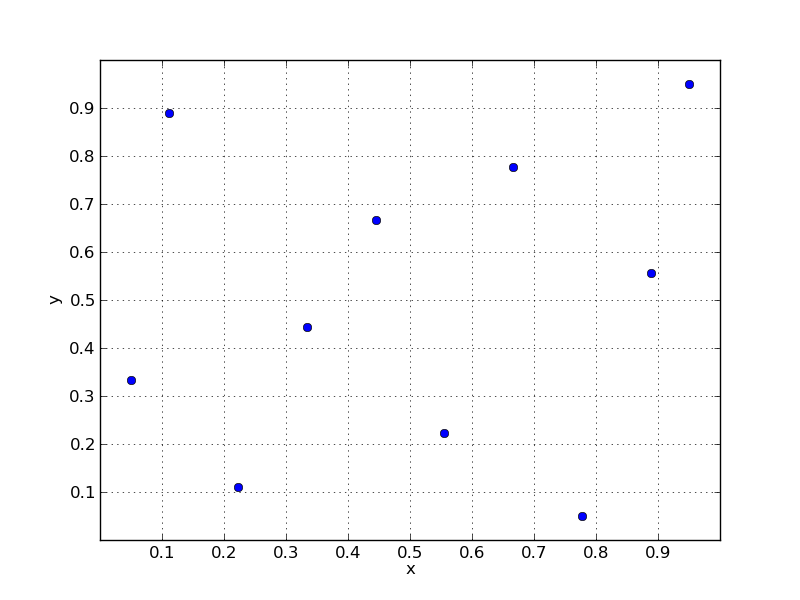
\includegraphics[width=0.58\textwidth]{./lhs.png}

\end{frame}
%%%%%%%%%%%%%%%%%%%%%%%%%%%%%%%%%%%%%%%%%%%%%%%%%%%%%%%%%%%%%%%%%%%%%%%%%%%%%%%%%%%%%%%%
\begin{frame}
\frametitle{Optimizing a LHS Plan}

\begin{itemize}
  \item The maximin metric describe by Morris and Mitchell makes use of two notions in an attempt to quantify the 'space-fillingness' of a sampling plan. 
  \item Unique distances between all points in the plan sorted in ascending order $\lbrace d_1, d_2, ..., d_m\rbrace$.
  \item Corresponding number of occurrences of each distance $\lbrace J_1, J_2, ..., J_m\rbrace$.  
  \item In words, the Morris and Mitchell criteria states that an optimized sampling plan will minimize all $J_i$ while maximizing the corresponding $d_i$. 
  \item The maximin sampling plan maximizes $d_1$, and among plans for which this is true, minimizes $J_1$, among plans for which this is true, maximizes $d_2$,....
\end{itemize}

\end{frame}
%%%%%%%%%%%%%%%%%%%%%%%%%%%%%%%%%%%%%%%%%%%%%%%%%%%%%%%%%%%%%%%%%%%%%%%%%%%%%%%%%%%%%%%%
\begin{frame}
\frametitle{Optimizing a LHS Plan}

\begin{itemize}
  \item The previous definition can be restated into a pseudo equivalent minimization problem.
\begin{equation}
\label{eq:Phi_q}
   \Phi_q(\textbf{X}) = \left(\sum_{j=1}^m J_j d_j^{-q} \right)^{1/q} \nonumber
\end{equation}
  \item The minimization of this equation and the Morris and Mitchell definition of the maximin sampling plan are used in unison to obtain a locally optimal sampling plan.
  \item Generate initial sampling plan, optimize for set of $q$ values using simulated annealing.  
  \item Resulting set of plans are contested directly against each other by explicit application of Morris and Mitchell's maximin definition. 
\end{itemize}

\end{frame}
%%%%%%%%%%%%%%%%%%%%%%%%%%%%%%%%%%%%%%%%%%%%%%%%%%%%%%%%%%%%%%%%%%%%%%%%%%%%%%%%%%%%%%%%
\begin{frame}
\frametitle{Kriging on a Sampling Plan}

\begin{itemize}
  \item Optimized sampling plan $\textbf{X}=\lbrace \textbf{x}^{(1)}, \textbf{x}^{(2)}, ... \textbf{x}^{(n)}\rbrace$. 
  \item At each datum $\textbf{x}^{(k)}$ a random process $Y(\textbf{x}^{(k)})$ induces an observation $y^{(k)}$.
  \item Resulting random field can be described with a mean value of $\textbf{1}\mu$ and a correlation matrix,
\begin{equation}
 \boldsymbol{\Psi} =
 \begin{pmatrix} 
	cor[Y(\textbf{x}^{(1)}), Y(\textbf{x}^{(1)})] & \cdots & 
		cor[Y(\textbf{x}^{(1)}), Y(\textbf{x}^{(n)})] \\
	\vdots & \ddots & \vdots \\ 
	cor[Y(\textbf{x}^{(n)}), Y(\textbf{x}^{(1)})] & \cdots & 
		cor[Y(\textbf{x}^{(n)}), Y(\textbf{x}^{(n)})]
 \end{pmatrix} \nonumber
\end{equation}  
\begin{equation}
   cor[Y(\textbf{x}^{(i)}), Y(\textbf{x}^{(l)})] = 
    \exp\left(-\sum_{j=1}^k \theta_j |x_j^{(i)} - x_j^{(l)} |^{p_j} \right) \nonumber
\end{equation}
\end{itemize}

\end{frame}
%%%%%%%%%%%%%%%%%%%%%%%%%%%%%%%%%%%%%%%%%%%%%%%%%%%%%%%%%%%%%%%%%%%%%%%%%%%%%%%%%%%%%%%%
\begin{frame}
\frametitle{Kriging on a Sampling Plan}

\begin{itemize}
  \item Given the formulation of the observations occurring at $\textbf{x}^{(k)}$ as instances of a stochastic process, the likelihood of seeing the observed data is,
\begin{eqnarray}
   L\left(\textbf{Y}^{(1)}, ..., \textbf{Y}^{(n)} | 
    \mu, \sigma, \lbrace \theta_1,..., \theta_k\rbrace, 
    \lbrace p_1,..., p_k\rbrace\right) = \nonumber \\
     \frac{1}{\left(2\pi\sigma^2\right)^{n/2}|\boldsymbol{\Psi}|^{1/2}}\times
     \exp\left[\frac{  \left(\textbf{y}-\textbf{1}\mu\right)^T
    \boldsymbol{\Psi}^{-1} \left(\textbf{y}-\textbf{1}\mu\right)}
    {2\sigma^2} \right] . \nonumber
\end{eqnarray} 
  \item Maximizing the log likelihood, 
   \begin{equation}
   	\hat{\mu} = \frac{ \textbf{1}^T\boldsymbol{\Psi}^{-1}\textbf{y} }
    		 	    {  \textbf{1}^T\boldsymbol{\Psi}^{-1}\textbf{1} } \nonumber
   \end{equation}
   \begin{equation}
   	\hat{\sigma}^2 = \frac{  \left(\textbf{y}-\textbf{1}\mu\right)^T
    			\boldsymbol{\Psi}^{-1} \left(\textbf{y}-\textbf{1}\mu\right)}{n}. \nonumber
   \end{equation}
\end{itemize}

\end{frame}
%%%%%%%%%%%%%%%%%%%%%%%%%%%%%%%%%%%%%%%%%%%%%%%%%%%%%%%%%%%%%%%%%%%%%%%%%%%%%%%%%%%%%%%%
\begin{frame}
\frametitle{Kriging on a Sampling Plan}

\begin{itemize}
  \item Substitute $\hat{\sigma}$ and $\hat{\mu}$ into log likelihood to get, concentrated ln-likelihood function.
   \begin{equation}
    \log(L) \approx -\frac{n}{2}\log\left(\hat{\sigma}^2\right) -
     \frac{1}{2} \log|\boldsymbol{\Psi}| \nonumber	
   \end{equation}
  \item Optimize with respect to the $\theta$ and $p$ parameters using global search algorithm.
  \item Once all optimizing parameters are available the goal is to utilize the parameters to build a model that makes function predictions on new points $\textbf{x}$.
\end{itemize}

\end{frame}
%%%%%%%%%%%%%%%%%%%%%%%%%%%%%%%%%%%%%%%%%%%%%%%%%%%%%%%%%%%%%%%%%%%%%%%%%%%%%%%%%%%%%%%%
\begin{frame}
\frametitle{Making Predictions with Kriging Surrogate}

\begin{itemize}
  \item Construct a vector of correlations with existing points and $\textbf{x}$,
   \begin{equation}
 	\boldsymbol{\psi} =
 	\begin{pmatrix} 
	 cor[Y(\textbf{x}^{(1)}), Y(\textbf{x})] \\
	 \vdots \\ 
	 cor[Y(\textbf{x}^{(n)}), Y(\textbf{x})] 
    \end{pmatrix}. \nonumber
   \end{equation} 
  \item  New predictions can be made at $\textbf{x}$ using the maximum likelihood estimator,
   \begin{equation}
    \hat{y}(\textbf{x}) = \hat{\mu} + 
   	 \boldsymbol{\psi}^T\boldsymbol{\Psi}^{-1}
   	  \left(\textbf{y} - \textbf{1}\hat{\mu}\right). \nonumber
   \end{equation}
  \item Prediction using kriging works to estimate a function value at a certain point by computing a weighted average of known function values in the vicinity of the objective points.
\end{itemize}

\end{frame}
%%%%%%%%%%%%%%%%%%%%%%%%%%%%%%%%%%%%%%%%%%%%%%%%%%%%%%%%%%%%%%%%%%%%%%%%%%%%%%%%%%%%%%%%
\subsection{Collocation and anchored-ANOVA}

\begin{frame}
\frametitle{Collocation and anchored-ANOVA Algorithmic Overview}

\begin{itemize}
  \item anchored-ANOVA: Decompose objective function into functions of one variable $f(x_i)$, two variables $f(x_i, x_j)$, three variables $f(x_i, x_j, x_k)$ as needed.
  \item Collocation: For each component in the decomposition construct a polynomial interpolant by sampling objective function at pre-defined points.
  \item The pre-defined points are determined by Smolyak Sparse Grids, and a selection of quadrature abscissas (e.g. Newton-Cotes). 
  \item Combine interpolants in decomposition to get an effective surrogate. 
\end{itemize}

\end{frame}
%%%%%%%%%%%%%%%%%%%%%%%%%%%%%%%%%%%%%%%%%%%%%%%%%%%%%%%%%%%%%%%%%%%%%%%%%%%%%%%%%%%%%%%%
\begin{frame}
\frametitle{Numerical Interpolation in 1D}

\begin{itemize}
  \item First, pick a set of $m_i$ collocation points.   
  \item Evaluate objective function at all collocation points.
  \item Interpolated function is a linear expansion of some basis $a_j^i$ (e.g. Lagrange polynomials) with weights $f\left(x_j^i\right)$.  
\end{itemize}

\begin{equation} 
    U^i = \sum_{j=1}^{m_i} 
     f\left(x_j^i\right) a_j^i \nonumber
\end{equation}

\end{frame}
%%%%%%%%%%%%%%%%%%%%%%%%%%%%%%%%%%%%%%%%%%%%%%%%%%%%%%%%%%%%%%%%%%%%%%%%%%%%%%%%%%%%%%%%
\begin{frame}
\frametitle{Clenshaw-Curtis Collocation Points}

\begin{itemize}  
  \item Clenshaw-Curtis points consist of the extrema of Chebyshev polynomials. 
  \item $n + 1 $ abscissas can exactly integrate polynomials of degree $n$.
  \item Points have the advantage of being nested.
\end{itemize}
\begin{equation}
    x_{j}^{i} = \left\{
     \begin{array}{cr}
       \cos\frac{\pi(j-1)}{m_i-1}   & j=1,...,m_i \text{ if } i>1 \\
       0   &  j=1 \text{ if } i=1
     \end{array}
   \right. \nonumber
\end{equation} 
\begin{equation} 
    m_i = \left\{
     \begin{array}{cr}
      2^{i-1}+1   & i>1 \\
      1   & i=1
     \end{array}
    \right. \nonumber
\end{equation}

\end{frame}
%%%%%%%%%%%%%%%%%%%%%%%%%%%%%%%%%%%%%%%%%%%%%%%%%%%%%%%%%%%%%%%%%%%%%%%%%%%%%%%%%%%%%%%%
\begin{frame}
\frametitle{Basis Functions}

\begin{itemize}  
  \item Lagrange characteristic polynomials are plagued by the fact that each evaluation requires $\mathcal{O}(m_i^2)$ operations and often the computation is numerically unstable.
  \item Instead the barycentric form of Lagrange characteristic polynomials is used to form a basis. 
\begin{equation} 
    a_j^i = \left\{
     \begin{array}{cc}
      1   & \text{ if } i=1 \\
      \displaystyle \frac{\frac{w_j^i}{x-x_j^i} }
       {\sum_{j=0}^{m_i} 
        \frac{w_j^i}{x-x_j^i}}   & j=1,...,m_i \text{ for } i>1
     \end{array}
    \right. \nonumber
\end{equation}
  \item For Clenshaw-Curtis collocation points the barycentric weights are given by,
\begin{equation} 
    w_j^i = (-1)^{j+1}\delta_j^i \hspace{1 cm}
     \delta_j^i = \left\{
                   \begin{array}{cc}
                    .5   & j=1 \text{ or } j=m_i \\
                    1   & \text{ else }  
				   \end{array}
				  \right. . \nonumber                   
\end{equation}        
\end{itemize}

\end{frame}
%%%%%%%%%%%%%%%%%%%%%%%%%%%%%%%%%%%%%%%%%%%%%%%%%%%%%%%%%%%%%%%%%%%%%%%%%%%%%%%%%%%%%%%%
\begin{frame}
\frametitle{Expanding to Multivariate Interpolation}

\begin{itemize}  
  \item Combine 1D interpolation formulas using tensor products
  \item Suffers from "Curse of Dimensionality".
  \item Mitigate the curse using Smolyak Sparse Grids.        
\end{itemize}

\begin{equation} 
    \left(U^{i_1} \otimes\cdots\otimes U^{i_d}\right)\left(f\right) = 
     \sum_{j_1=1}^{m_{i_1}} \cdots
      \sum_{j_d=1}^{m_{i_d}} f\left(
       x_{j_1}^{i_1},\cdots,x_{j_d}^{i_d}\right)
        \left(a_{j_1}^{i_1}\otimes\cdots\otimes a_{j_d}^{i_d}\right) \nonumber
\end{equation} 

\end{frame}
%%%%%%%%%%%%%%%%%%%%%%%%%%%%%%%%%%%%%%%%%%%%%%%%%%%%%%%%%%%%%%%%%%%%%%%%%%%%%%%%%%%%%%%%
\begin{frame}
\frametitle{Smolyak Sparse Grids}

\begin{itemize}  
  \item Based on full tensor product formula the only difference being not all tensor products are used. 
  \item In explicit form, the Smolyak formula is,
\begin{equation} 
    A_{q,d}(f) = 
     \sum_{q-d+1\leq \vert \textbf{i}\vert\leq q}
      \left(-1\right)^{q-\vert\textbf{i}\vert}
       \binom{d-1}{q-\vert\textbf{i}\vert}
        \left(U^{i_1} \otimes\cdots\otimes U^{i_d}\right). \nonumber
\end{equation}  
  \item $i_k$ is the index corresponding to the level of interpolation in dimension $k$. 
  \item The magnitude of $\textbf{i}$ is $\vert\textbf{i}\vert = \vert i_1 +\cdots+ i_d\vert$. 
  \item $q$ keeps track of the level of interpolation of the Smolyak algorithm. More tensor product combinations are allowed as $q$ increases. 
  \item Smolyak algorithm reduces the total number of tensor product components by limiting the entries of $\textbf{i}$.     
\end{itemize}

\end{frame}
%%%%%%%%%%%%%%%%%%%%%%%%%%%%%%%%%%%%%%%%%%%%%%%%%%%%%%%%%%%%%%%%%%%%%%%%%%%%%%%%%%%%%%%%
\begin{frame}
\frametitle{Smolyak Sparse Grid Visualization}

\begin{columns}
 \begin{column}{0.5\textwidth}
  \centering
  Level 4 Clenshaw-Curtis Full Tensor Product Grid
  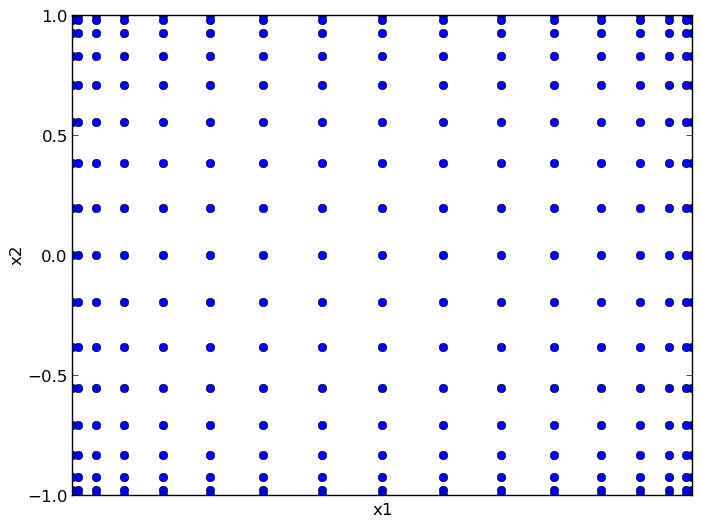
\includegraphics[width=1.\textwidth]{./tensor_prod_grid_L4.png}
 \end{column}
 \begin{column}{0.5\textwidth}
  \centering
  Level 4 Clenshaw-Curtis Smolyak Sparse Grid
  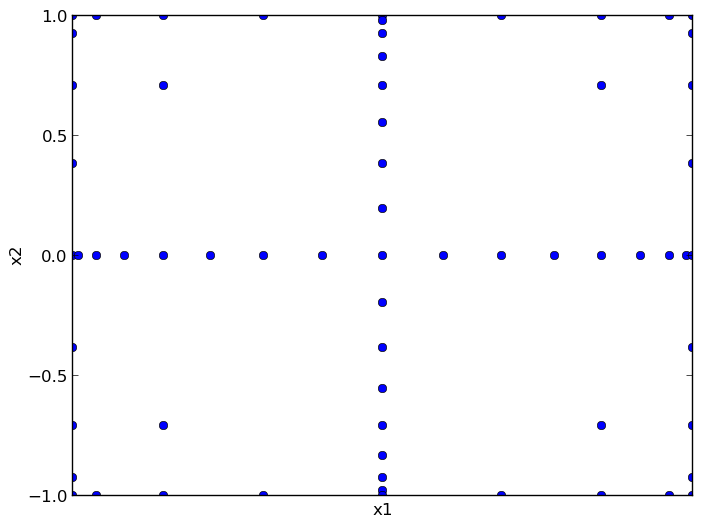
\includegraphics[width=1.\textwidth]{./sparse_grid_L4.png}
 \end{column}
\end{columns}

\end{frame}
%%%%%%%%%%%%%%%%%%%%%%%%%%%%%%%%%%%%%%%%%%%%%%%%%%%%%%%%%%%%%%%%%%%%%%%%%%%%%%%%%%%%%%%%
\begin{frame}

\frametitle{Smolyak Sparse Grid Visualization}
\centering
Level 0 Sparse Grid
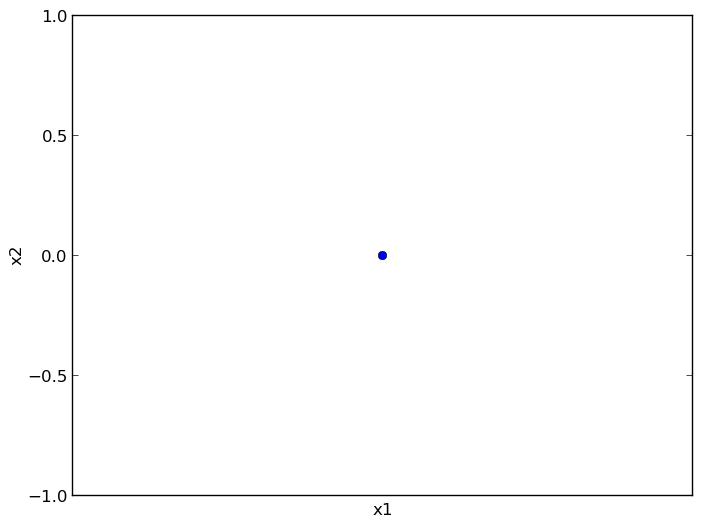
\includegraphics[width=.75\textwidth]{./sparse_grid_L0.png}

\end{frame}
%%%%%%%%%%%%%%%%%%%%%%%%%%%%%%%%%%%%%%%%%%%%%%%%%%%%%%%%%%%%%%%%%%%%%%%%%%%%%%%%%%%%%%%%
\begin{frame}

\frametitle{Smolyak Sparse Grid Visualization}
\centering
Level 1 Sparse Grid
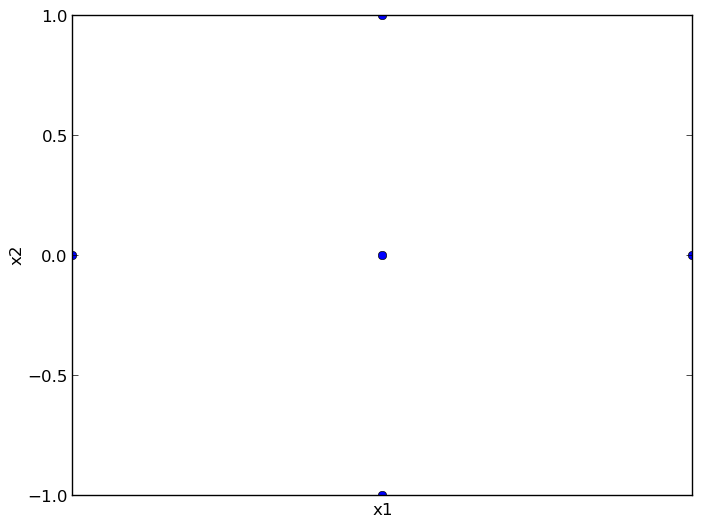
\includegraphics[width=.75\textwidth]{./sparse_grid_L1.png}

\end{frame}
%%%%%%%%%%%%%%%%%%%%%%%%%%%%%%%%%%%%%%%%%%%%%%%%%%%%%%%%%%%%%%%%%%%%%%%%%%%%%%%%%%%%%%%%
\begin{frame}

\frametitle{Smolyak Sparse Grid Visualization}
\centering
Level 2 Sparse Grid
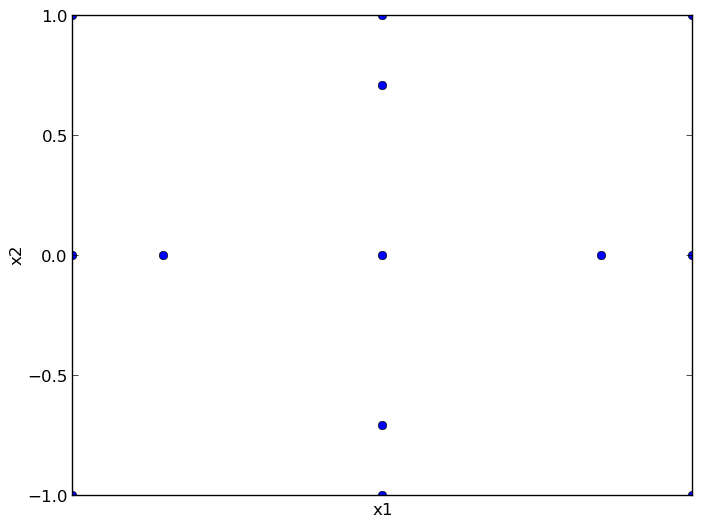
\includegraphics[width=.75\textwidth]{./sparse_grid_L2.png}

\end{frame}
%%%%%%%%%%%%%%%%%%%%%%%%%%%%%%%%%%%%%%%%%%%%%%%%%%%%%%%%%%%%%%%%%%%%%%%%%%%%%%%%%%%%%%%%
\begin{frame}

\frametitle{Smolyak Sparse Grid Visualization}
\centering
Level 3 Sparse Grid
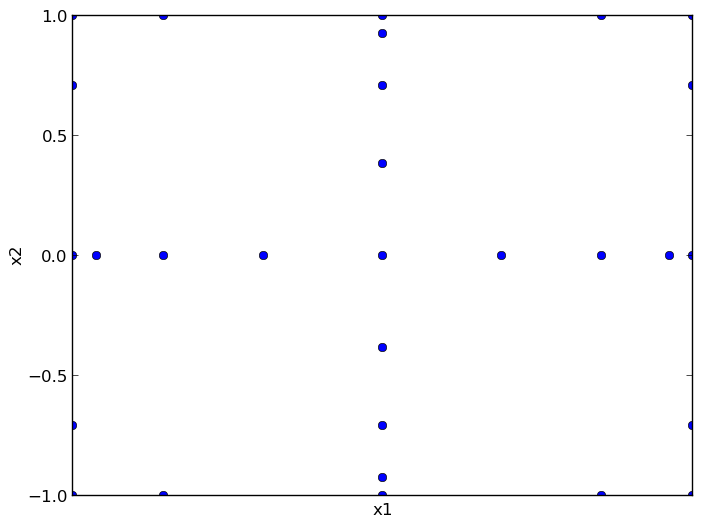
\includegraphics[width=.75\textwidth]{./sparse_grid_L3.png}

\end{frame}
%%%%%%%%%%%%%%%%%%%%%%%%%%%%%%%%%%%%%%%%%%%%%%%%%%%%%%%%%%%%%%%%%%%%%%%%%%%%%%%%%%%%%%%%
\begin{frame}

\frametitle{Smolyak Sparse Grid Visualization}
\centering
Level 4 Sparse Grid
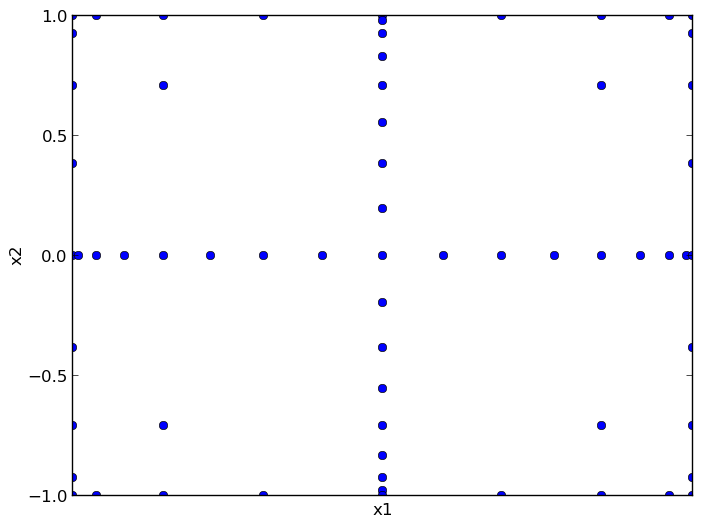
\includegraphics[width=.75\textwidth]{./sparse_grid_L4.png}

\end{frame}
%%%%%%%%%%%%%%%%%%%%%%%%%%%%%%%%%%%%%%%%%%%%%%%%%%%%%%%%%%%%%%%%%%%%%%%%%%%%%%%%%%%%%%%%
\begin{frame}

\frametitle{Smolyak Sparse Grid Visualization}
\centering
Level 5 Sparse Grid
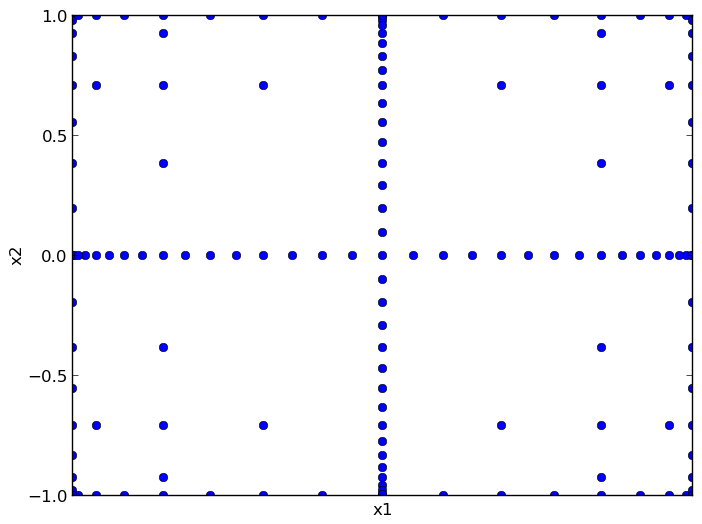
\includegraphics[width=.75\textwidth]{./sparse_grid_L5.png}

\end{frame}
%%%%%%%%%%%%%%%%%%%%%%%%%%%%%%%%%%%%%%%%%%%%%%%%%%%%%%%%%%%%%%%%%%%%%%%%%%%%%%%%%%%%%%%%
\begin{frame}

\frametitle{Smolyak Sparse Grid Visualization}
\centering
Level 6 Sparse Grid
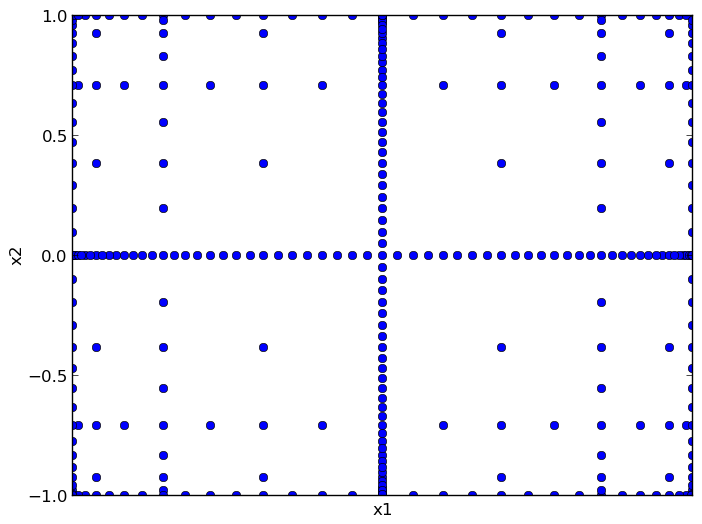
\includegraphics[width=.75\textwidth]{./sparse_grid_L6.png}

\end{frame}
%%%%%%%%%%%%%%%%%%%%%%%%%%%%%%%%%%%%%%%%%%%%%%%%%%%%%%%%%%%%%%%%%%%%%%%%%%%%%%%%%%%%%%%%
\begin{frame}

\frametitle{Smolyak Sparse Grid Visualization}
\centering
Level 7 Sparse Grid
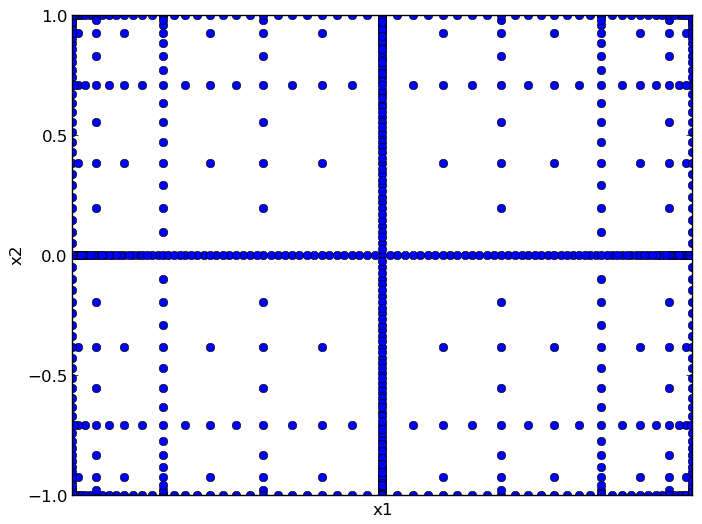
\includegraphics[width=.75\textwidth]{./sparse_grid_L7.png}

\end{frame}
%%%%%%%%%%%%%%%%%%%%%%%%%%%%%%%%%%%%%%%%%%%%%%%%%%%%%%%%%%%%%%%%%%%%%%%%%%%%%%%%%%%%%%%%
\begin{frame}
\frametitle{Recursive Definition of Smolyak's Algorithm}

\begin{itemize}
  \item The explicit definition of Smolyak's algorithm can be rewritten in a recursive fashion.
  \item Able to increase interpolation level without having to start over each time.
  \item Hierarchical surplus serves as an error indicator. Lets you know how well the interpolation is going as the grid is refined.
  \item Use hierarchical surplus to determine convergence.
\end{itemize}

\begin{equation}
 A_{q,d}(f) = A_{q-1,d}(f) + \Delta A_{q,d} \nonumber
\end{equation}
\begin{equation} 
 \Delta A_{q,d} = \sum_{\vert\textbf{i}\vert=q}
  \left( \underbrace{f(x_{j_1}^{i_1},...,x_{j_d}^{i_d}) - 
   A_{q-1,d}(x_{j_1}^{i_1},...,x_{j_d}^{i_d}}_{\text{Hierarchical Surplus}})\right)\cdot
    \left(a_{j_1}^{i_1}\otimes\cdots\otimes a_{j_d}^{i_d}\right) \nonumber
\end{equation}

\end{frame}
%%%%%%%%%%%%%%%%%%%%%%%%%%%%%%%%%%%%%%%%%%%%%%%%%%%%%%%%%%%%%%%%%%%%%%%%%%%%%%%%%%%%%%%%
\begin{frame}
\frametitle{anchored-ANOVA Decomposition}

\begin{itemize}
  \item Consider a $d$-dimensional function $f(\textbf{x}) = f(x_1, x_2, ..., x_d)$.
  \item The operator $P_{\textbf{u}}$ projects from a $d$-dimensional space to a $\vert\textbf{u}\vert$-dimensional space for some set $\textbf{u}\subseteq \mathcal{D} = \lbrace 1,...,d\rbrace$.  
\begin{equation}
 f_{\textbf{u}}(\textbf{x}_{\textbf{u}}) = P_{\textbf{u}}f\left(\textbf{x}\right) =
  \int_{\Omega^{d-\vert\textbf{u}\vert}} 
   f\left(\textbf{x}\right)d\mu_{\mathcal{D}\setminus\textbf{u}}
    \left(\textbf{x}\right) \nonumber
\end{equation}
  \item Use the Dirac measure $\delta(\textbf{x}-\textbf{a})d\textbf{x}$ to evaluate the projection operator at an "anchor" point $\textbf{a}$,
\begin{equation} 
 P_{\textbf{u}}f\left(\textbf{x}\right) = 
  f\left(\textbf{x}\right)\vert_{\textbf{x}=
   \textbf{a}\setminus\textbf{x}_{\textbf{u}}}. \nonumber
\end{equation}
  \item For $\textbf{u}\neq\textbf{v}$ the following orthogonality relation holds:
\begin{equation} 
 \left(f_{\textbf{u}},f_{\textbf{v}}\right) = 0 \nonumber
\end{equation}
\end{itemize}

\end{frame}
%%%%%%%%%%%%%%%%%%%%%%%%%%%%%%%%%%%%%%%%%%%%%%%%%%%%%%%%%%%%%%%%%%%%%%%%%%%%%%%%%%%%%%%%
\begin{frame}
\frametitle{anchored-ANOVA Decomposition}

\begin{itemize}
  \item A function can be written in terms of its $2^d$ orthogonal components,
\begin{equation} 
 f\left(\textbf{x}\right) = 
  \sum_{\textbf{u}\subseteq\mathcal{D}}
   f_{\textbf{u}}\left(\textbf{x}_{\textbf{u}}\right). \nonumber
\end{equation}
  \item The component functions $f_{\textbf{u}}$ are defined recursively,
\begin{equation} 
 f_{\textbf{u}}\left(\textbf{x}_{\textbf{u}}\right) = 
  P_{\textbf{u}}f\left(\textbf{x}\right) -
   \sum_{\textbf{v}\subset\textbf{u}}
    f_{\textbf{v}}\left(\textbf{x}_{\textbf{v}}\right). \nonumber 
\end{equation}
  \item Zeroth order component: 
\begin{align*}
 f_{\lbrace \emptyset \rbrace} = f(\overline{\textbf{x}}) 
\end{align*}
  \item First and second order components:
\begin{align*}
 f_{\lbrace x_i \rbrace} &= f\left(\textbf{x}\right)\vert_{\textbf{x} =
   \textbf{a}\setminus x_i} - f_{\lbrace \emptyset \rbrace} \\
 f_{\lbrace x_i, x_j \rbrace} &= f\left(\textbf{x}\right)\vert_{\textbf{x}=
   \textbf{a}\setminus \lbrace x_i, x_j \rbrace} - f_{\lbrace \emptyset \rbrace} -
    f_{\lbrace x_i \rbrace} - f_{\lbrace x_j \rbrace} 
\end{align*}
\end{itemize}

\end{frame}
%%%%%%%%%%%%%%%%%%%%%%%%%%%%%%%%%%%%%%%%%%%%%%%%%%%%%%%%%%%%%%%%%%%%%%%%%%%%%%%%%%%%%%%%
\begin{frame}
\frametitle{Note on anchored-ANOVA and Taylor Series}

\begin{itemize}
  \item The multivariate Taylor series of $f(\textbf{x})$ about $\textbf{\=x}$,
\begin{align*} 
 f\left(\textbf{x}\right) = 
  f\left(\bar{\textbf{x}}\right) &+
   \sum_{i=1}^{d} 
    \frac{\partial f(\textbf{x})}{\partial x_i}\left(x_i - \bar{x}_i\right) \\
     &+ \frac{1}{2!}\sum_{i,j=1}^{d}
      \frac{\partial^2 f(\textbf{x})}{\partial x_i\partial x_j}
       \left(x_i - \bar{x}_i\right) \left(x_j - \bar{x}_j\right) + ...
\end{align*}  
  \item Evaluate at $\textbf{x} = \textbf{a}\setminus x_i$,
\begin{align*} 
    f\left(\textbf{x}\right)\vert_{\textbf{x} = \textbf{a}\setminus x_i} = 
     f\left(\bar{\textbf{x}}\right) +
      \frac{\partial f(\textbf{x})}{\partial x_i}\left(x_i - \bar{x}_i\right)
       + \frac{1}{2!} \frac{\partial^2 f(\textbf{x})}{\partial x_i^2}
        \left(x_i - \bar{x}_i\right)^2 + ...
\end{align*}
  \item Component functions are entire Taylor series expansions.
  \item Truncated anchored-ANOVA expansion will always be a better approximation than a truncated Taylor expansion. 
      
\end{itemize}

\end{frame}
%%%%%%%%%%%%%%%%%%%%%%%%%%%%%%%%%%%%%%%%%%%%%%%%%%%%%%%%%%%%%%%%%%%%%%%%%%%%%%%%%%%%%%%%
\begin{frame}
\frametitle{Combining anchored-ANOVA and Smolyak Sparse Grids}

\begin{itemize}
  \item anchored-ANOVA decomposition forms foundation for surrogate model.
  \item Build each component function on a Smolyak sparse grid.
  \item Build all first-order components first. 
  \item Compute sensitivity coefficient for each component. 
\begin{equation} 
 \eta_i = \frac{
  \int_{\Omega_i}
   \left[f(\textbf{x})\vert_{
    \textbf{x}=\overline{\textbf{x}}\setminus x_i}
     -f(\overline{\textbf{x}}) \right]\rho(x_i)dx_i}
      {
       f_{\left\{\emptyset\right\}}} \nonumber
\end{equation}
  \item Build higher order components for only those variables whose sensitivity coefficients  exceed a certain threshold.
  \item Continue to add higher order terms until convergence criteria met.     
\end{itemize}

\end{frame}
%%%%%%%%%%%%%%%%%%%%%%%%%%%%%%%%%%%%%%%%%%%%%%%%%%%%%%%%%%%%%%%%%%%%%%%%%%%%%%%%%%%%%%%%

% APPLICATION OF SURROGATE METHODS
\section{Application of Surrogate Models}

\subsection{Infinite Lattice}
%%%%%%%%%%%%%%%%%%%%%%%%%%%%%%%%%%%%%%%%%%%%%%%%%%%%%%%%%%%%%%%%%%%%%%%%%%%%%%%%%%%%%%%%
\begin{frame}
\frametitle{Infinite Lattice Problem Statement}

\begin{itemize}
  \item Reactor of infinite size is considered, effectively removing the effects of geometry in neutron transport
  \item System entirely characterized in terms of its material properties.
  \item Analytic solution available!       
\end{itemize}

\begin{equation}
   \left(
    \begin{array}{cc}
     \Sigma_{a_1} + \Sigma_{1\rightarrow 2} & 0 \\
     -\Sigma_{12} & \Sigma_{a_2} 
    \end{array}
   \right)
   \left(
    \begin{array}{c}
     \phi_1 \\
     \phi_2
    \end{array}
   \right) 
   = \frac{1}{k_{\infty}}
   \left(
    \begin{array}{cc}
     \nu\Sigma_{f_1} & \nu\Sigma_{f_2} \\
     0 & 0 
    \end{array}
   \right)
   \left(
    \begin{array}{c}
     \phi_1 \\
     \phi_2
    \end{array}
   \right) \nonumber
\end{equation}
\begin{equation}
   k_{\infty} = \frac{\Sigma_{a_2}\nu\Sigma_{f_1} + 
             \Sigma_{1\rightarrow 2}\nu\Sigma_{f_2}}{
              \Sigma_{a_2}\left(
               \Sigma_{a_1} + \Sigma_{1\rightarrow 2}\right)} \nonumber
\end{equation}  

\end{frame}
%%%%%%%%%%%%%%%%%%%%%%%%%%%%%%%%%%%%%%%%%%%%%%%%%%%%%%%%%%%%%%%%%%%%%%%%%%%%%%%%%%%%%%%%
\begin{frame}
\frametitle{Infinite Lattice Problem Statement}

\begin{itemize}
  \item Assume all variation in $k_{\infty}$ can be attributed to its input cross sections, whose distributions follow a multivariate Gaussian.       
\end{itemize}

\begin{table}[H]
\centering
\resizebox{\textwidth}{!}{%
\begin{tabular}{||c||c|c|c|c|c|c|c||} 
\hline \hline
  &  &  & \multicolumn{5}{|c||}{\textbf{Correlation Coefficient Matrix}}  \\ \hline
  & \textbf{Mean} & \textbf{Standard Dev.} & $\Sigma_{a_1}$ & $\Sigma_{a_2}$ & 
  $\nu\Sigma_{f_1}$ & $\nu\Sigma_{f_2}$ & $\Sigma_{1\rightarrow 2}$ \\ \hline \hline
$\Sigma_{a_1}$ & 1.04E-02 & 9.06E-05 & 1 & 0.07 & -0.13 & 0.02 & 0.75 \\ \hline
$\Sigma_{a_2}$ & 1.10E-01 & 2.31E-04 & 0.07  &  1     & 0.06  & 0.31 & -0.07 \\ \hline
$\nu\Sigma_{f_1}$ & 9.00E-03 & 4.85E-05 & -0.13 &  0.06  & 1     & 0.33 & -0.10 \\ \hline
$\nu\Sigma_{f_2}$ & 1.91E-01 & 8.87E-04 & 0.02  &  0.31  & 0.33  & 1    & 0.01 \\ \hline
$\Sigma_{1\rightarrow 2}$ & 1.80E-02 & 2.18E-04 & 0.75  &  -0.07 & -0.10 & 0.01 & 1 \\ \hline \hline
\end{tabular}}
\end{table}

\end{frame}
%%%%%%%%%%%%%%%%%%%%%%%%%%%%%%%%%%%%%%%%%%%%%%%%%%%%%%%%%%%%%%%%%%%%%%%%%%%%%%%%%%%%%%%%
\begin{frame}
\frametitle{Infinite Lattice Problem Objective}

\begin{itemize}
  \item Propagate cross section uncertainties to find the mean and standard deviation of $k_{\infty}$ using Monte Carlo sampling of true and surrogate functions, and the "Sandwich Equation".
\begin{align*}
 \sigma^2(k_{\infty}) = S^TCS
\end{align*} 
\begin{equation}
 S^T = \left(
  \begin{array}{ccccc}
   \frac{\partial k_{\infty}}{\partial\Sigma_{a_1}} &
    \frac{\partial k_{\infty}}{\partial\Sigma_{a_2}} &
     \frac{\partial k_{\infty}}{\partial\nu\Sigma_{f_1}} &
      \frac{\partial k_{\infty}}{\partial\nu\Sigma_{f_2}} &
       \frac{\partial k_{\infty}}{\partial\Sigma_{1\rightarrow 2}}
 \end{array}\right) \nonumber
\end{equation} 
  \item Also, find sensitivity coefficients analytically and numerically.
\begin{equation}
 \frac{\partial k_{\infty}}{\partial \Sigma_i}\biggr\rvert_
  {\Sigma_{j\neq i} = \bar{\Sigma}_j}
   \approx \frac{k_{\infty}(\Sigma_i + \Delta\Sigma_i) - 
    k_{\infty}(\Sigma_i - \Delta\Sigma_i)}
     {2\Delta\Sigma_i} \nonumber
\end{equation}        
           
\end{itemize}

\end{frame}
%%%%%%%%%%%%%%%%%%%%%%%%%%%%%%%%%%%%%%%%%%%%%%%%%%%%%%%%%%%%%%%%%%%%%%%%%%%%%%%%%%%%%%%%
\begin{frame}
\frametitle{Convergence of 5-D Sparse Grid Interpolant}

\begin{columns}
 \begin{column}{0.5\textwidth}
  \centering
  Hierarchical Surplus  
  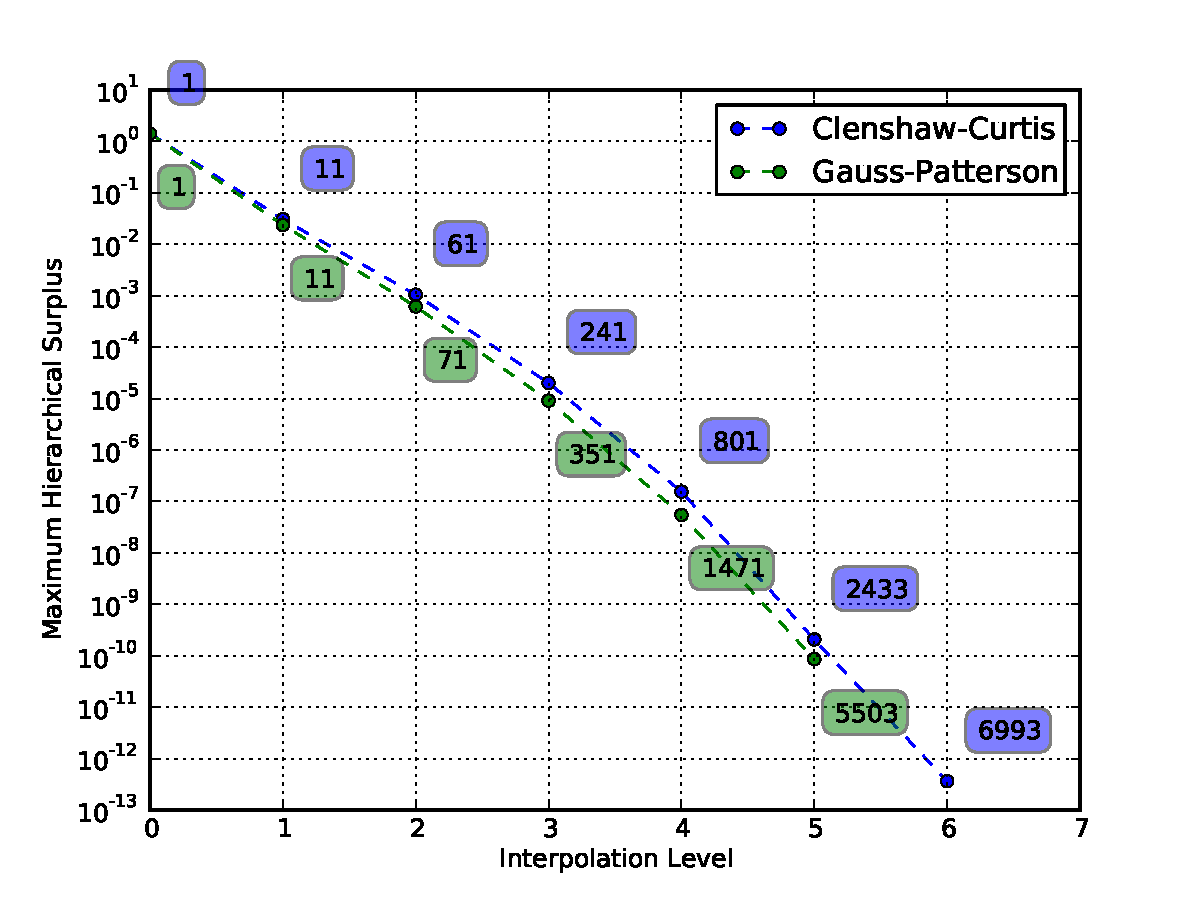
\includegraphics[width=1.\textwidth]{./kinf_sparse_grid_convergence.pdf}
 \end{column}
 \begin{column}{0.5\textwidth}
  \centering
  Number of Abscissas 
  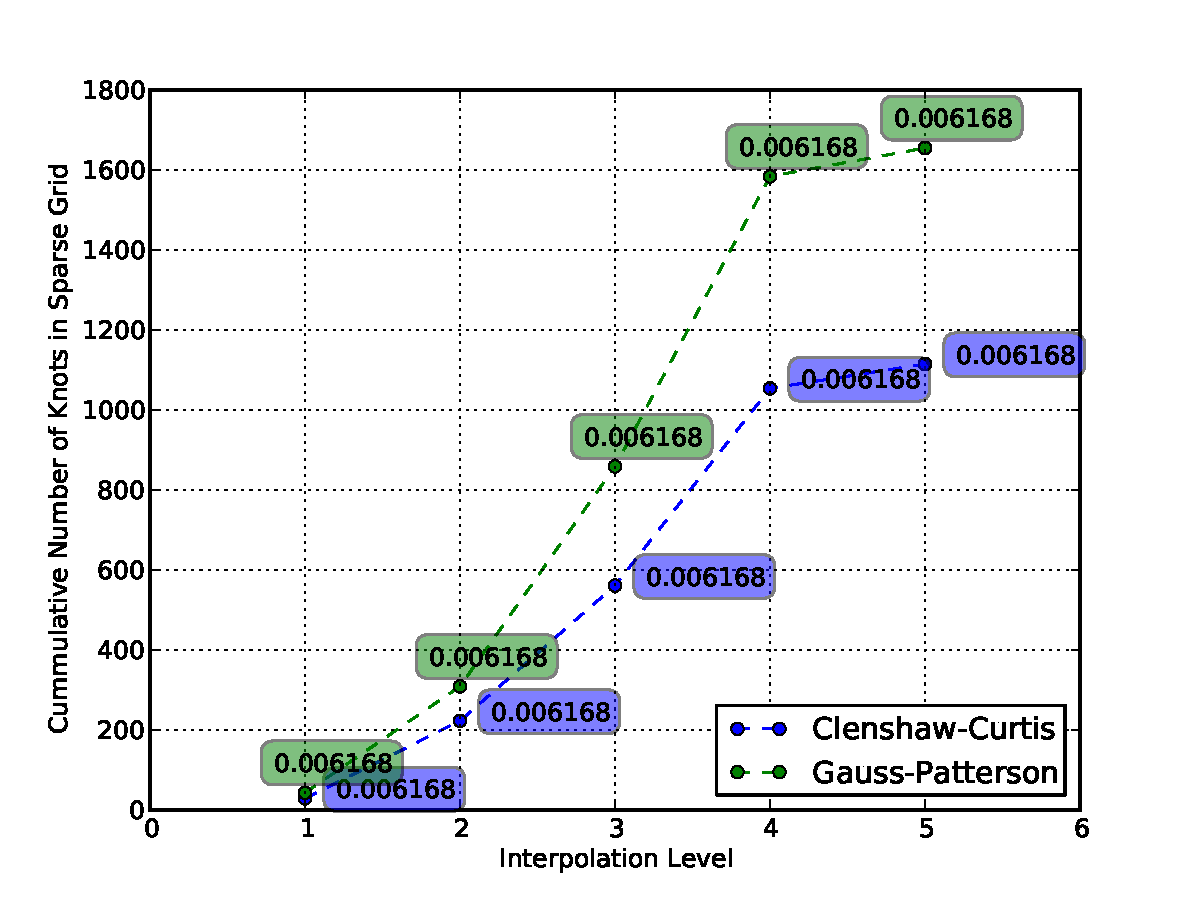
\includegraphics[width=1.\textwidth]{./kinf_sparse_grid_numknots.pdf}
 \end{column}
\end{columns}

\end{frame}
%%%%%%%%%%%%%%%%%%%%%%%%%%%%%%%%%%%%%%%%%%%%%%%%%%%%%%%%%%%%%%%%%%%%%%%%%%%%%%%%%%%%%%%%
\begin{frame}
\frametitle{Mean and Variance of $k_{\infty}$}

\begin{itemize}
  \item 1000 Monte Carlo samples, using the same random numbers, were gathered for each method.
  \item In "1D ANOVA" only the 5 first-order components are used.
  \item In "All ANOVA" all 32 components are used.
  \item Clenshaw-Curtis collocation points represented by "CC" while "GP" is Gauss-Patterson.
\end{itemize}
\begin{table} 
\centering
\resizebox{\textwidth}{!}{%
\begin{tabular}{||c|c|c|c|c||} 
\hline \hline
\textbf{Method} & \textbf{Mean} & \textbf{99\% CI} & \textbf{Standard Dev.} & \textbf{99\% CI} \\ \hline
5D Sparse Grid CC      & 1.41562 & (1.41512, 1.41612) & 0.006168 & (0.005909, 0.006544) \\ \hline
5D Sparse Grid GP      & 1.41562 & (1.41512, 1.41612) & 0.006168 & (0.005831, 0.006544) \\ \hline
1D ANOVA CC  & 1.41560 & (1.41510, 1.41610) & 0.006168 & (0.005831, 0.006544) \\ \hline
All ANOVA CC & 1.41562 & (1.41512, 1.41612) & 0.006168 & (0.005831, 0.006544) \\ \hline
1D ANOVA GP  & 1.41560 & (1.41510, 1.41610) & 0.006168 & (0.005831, 0.006544) \\ \hline
All ANOVA GP & 1.41562 & (1.41512, 1.41612) & 0.006168 & (0.005831, 0.006544) \\ \hline
True Function & 1.41562 & (1.41512, 1.41612) & 0.006168 & (0.005831, 0.006544) \\ \hline
Sandwich               &         &                    & 0.006540 &                      \\
\hline \hline
\end{tabular}}
\end{table}

\end{frame}
%%%%%%%%%%%%%%%%%%%%%%%%%%%%%%%%%%%%%%%%%%%%%%%%%%%%%%%%%%%%%%%%%%%%%%%%%%%%%%%%%%%%%%%%
\begin{frame}
\frametitle{Sensitivity Coefficients for $k_{\infty}$}

\begin{itemize}
  \item Central differencing... perturbations (1\%) made to each cross section while holding the others at mean value. 
  \item Models differ from analytic coefficients in fourth decimal place
  \item Expected due to $\mathcal{O}(\Delta\Sigma^2)$ convergence of central differencing.
\end{itemize}

\begin{table}
\centering
\resizebox{\textwidth}{!}{%
\begin{tabular}{||c|c|c|c|c|c||} 
\hline \hline
  & \multicolumn{5}{|c||}{\textbf{Normalized Sensitivity Coefficient of $k_{\infty}$}}  \\ \hline
\textbf{Method} & $\Sigma_{a_1}$ & $\Sigma_{a_2}$ & $\nu\Sigma_{f_1}$ & $\nu\Sigma_{f_2}$ & $\Sigma_{1\rightarrow 2}$ \\ \hline
5D Sparse Grid CC  & -.367551 & -.776087 & .224060 & .776010 & .143491 \\ \hline
5D Sparse Grid GP  & -.367551 & -.776087 & .224060 & .776010 & .143491 \\ \hline
1D ANOVA CC        & -.367556 & -.776098 & .224063 & .776020 & .143493 \\ \hline
All ANOVA CC       & -.367551 & -.776087 & .224060 & .776010 & .143491 \\ \hline
1D ANOVA GP        & -.367556 & -.776098 & .224063 & .776020 & .143493 \\ \hline
All ANOVA GP       & -.367551 & -.776087 & .224060 & .776010 & .143491 \\ \hline
Analytic           & -.367520 & -.775956 & .224044 & .775956 & .143476 \\ \hline
Central Difference & -.367551 & -.776089 & .224060 & .776011 & .143492 \\
\hline \hline
\end{tabular}}
\end{table}

\end{frame}
%%%%%%%%%%%%%%%%%%%%%%%%%%%%%%%%%%%%%%%%%%%%%%%%%%%%%%%%%%%%%%%%%%%%%%%%%%%%%%%%%%%%%%%%
\begin{frame}
\frametitle{Kriging Surrogate for $k_{\infty}$}

\begin{itemize}
  \item Observe that for ten evaluation points, twice the number of design variables in the objective function, error goes to zero. 
\end{itemize}

\begin{figure}
 \begin{center}
  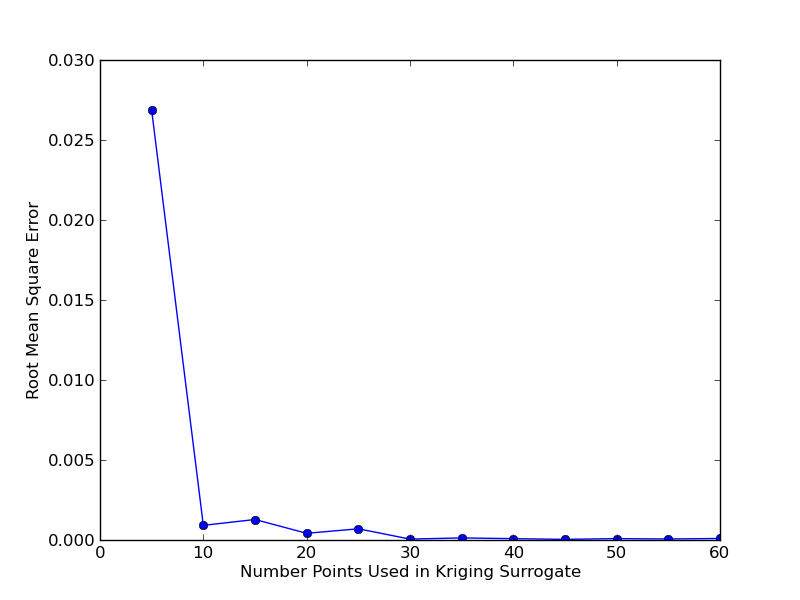
\includegraphics[width=.75\textwidth]{./error_vs_npoints.png}
 \end{center}
\end{figure}

\end{frame}
%%%%%%%%%%%%%%%%%%%%%%%%%%%%%%%%%%%%%%%%%%%%%%%%%%%%%%%%%%%%%%%%%%%%%%%%%%%%%%%%%%%%%%%%
\subsection{Point Kinetics/Lumped TH}

\begin{frame}
\frametitle{Point Kinetics/Lumped Thermal Hydraulics Problem Statement}

\begin{itemize}
  \item Modeling a transient resulting from a half sawtooth external reactivity insertion in a BN800 sodium fast cooled reactor.
\begin{equation}
 \rho_{ex}(t) = \left\{
  \begin{array}{cr}
   t\rho_{max}/20 & t \leq 20 \\
    0                      & t > 20 
    \end{array}
    \right. \nonumber
\end{equation}     
  \item The physical model of the reactor consists of point kinetics to model the neutronics and lumped thermal hydraulics equations to describe temperature feedback. 
  \item The coupled system is nonlinear and only has a time dependence.
  \item Kinetics coupled to thermal hydraulics through reactivity. 
\end{itemize}

\begin{equation}
 \rho(T_f,T_c,t) = \rho_{ex} + \alpha_d(T_f - T_f(0))
    + \alpha_c(T_c - T_c(0)) \nonumber
\end{equation}

\end{frame}
%%%%%%%%%%%%%%%%%%%%%%%%%%%%%%%%%%%%%%%%%%%%%%%%%%%%%%%%%%%%%%%%%%%%%%%%%%%%%%%%%%%%%%%%
\begin{frame}
\frametitle{Point Kinetics/Lumped Thermal Hydraulics Problem Statement}

\begin{figure}
 \begin{center}
  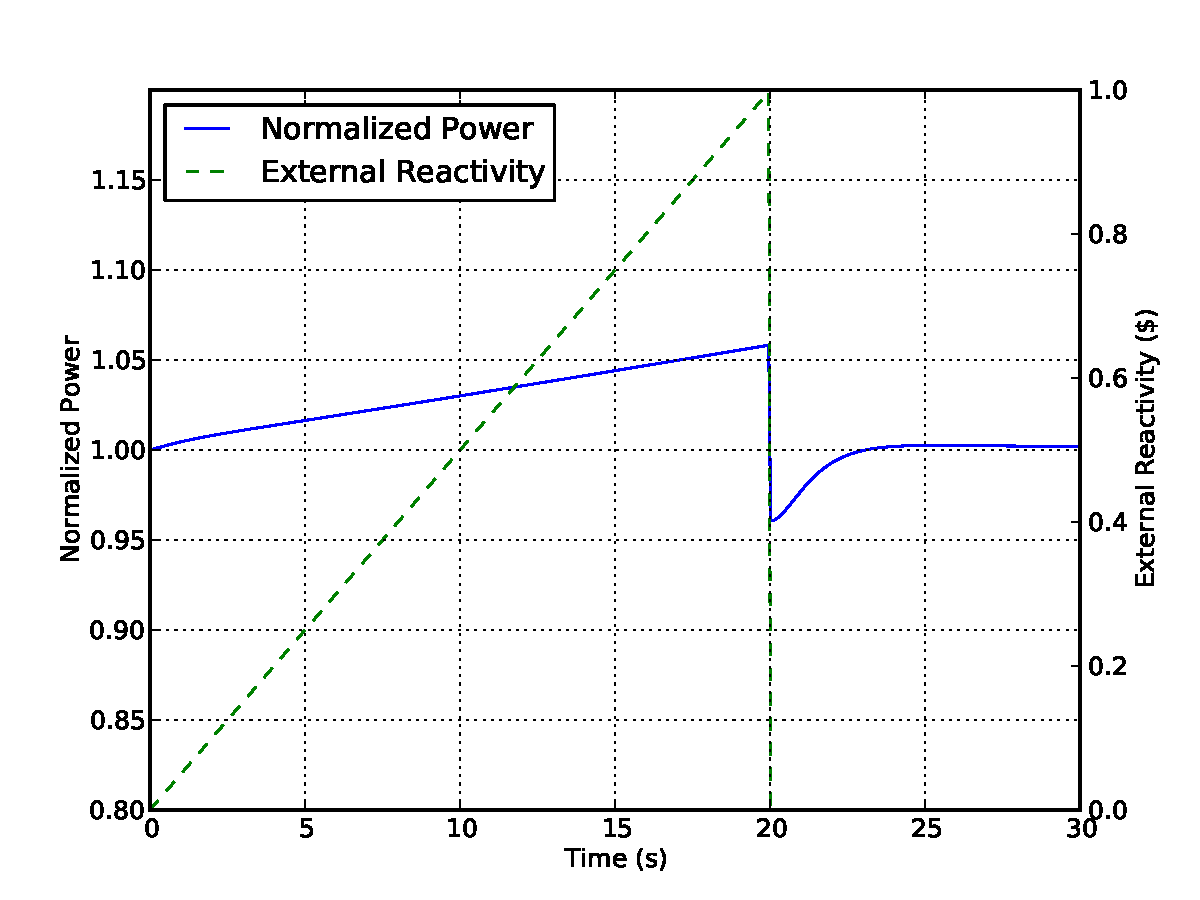
\includegraphics[width=.9\textwidth]{./pk_power.pdf}
 \end{center}
\end{figure}

\end{frame}
%%%%%%%%%%%%%%%%%%%%%%%%%%%%%%%%%%%%%%%%%%%%%%%%%%%%%%%%%%%%%%%%%%%%%%%%%%%%%%%%%%%%%%%%
\begin{frame}
\frametitle{Point Kinetics/Lumped Thermal Hydraulics Problem Statement}

\begin{itemize}
  \item Reactor Power
\begin{align*}
 \frac{dP}{dt} = \frac{\rho(T_f,T_c,t)-\beta}{\Lambda}P +
  \sum_{k=1}^6 \lambda_k C_k 
\end{align*}
  \item Precursor Concentration
\begin{align*}
 \frac{dC_k}{dt} = -\lambda_k C_k +
  \frac{\beta_k}{\Lambda}P
\end{align*}
  \item Fuel Temperature
\begin{align*}
  M_f c_{pf}\frac{dT_f}{dt} = P + Ah(T_c-T_f)
\end{align*} 
  \item Coolant Temperature
\begin{align*}
 M_c c_{pc}\left(\frac{dT_c}{dt} +v \frac{T_c - T_{in}}{L}\right) = 
  Ah(T_f-T_c)
\end{align*} 
\end{itemize}

\end{frame}
%%%%%%%%%%%%%%%%%%%%%%%%%%%%%%%%%%%%%%%%%%%%%%%%%%%%%%%%%%%%%%%%%%%%%%%%%%%%%%%%%%%%%%%%
\begin{frame}
\frametitle{Point Kinetics/Lumped Thermal Hydraulics Objective}

\begin{itemize}
  \item A total of twenty two random variables will be investigated for their affect on the maximum fuel temperature attained during transient.
\begin{align*}
 \lambda_1, \lambda_2, \lambda_3, \lambda_4, \lambda_5, \lambda_6, \beta_1, \beta_2, \beta_3, \beta_4, \beta_5, \beta_6 \\
 \Lambda, Ah, M_c, M_f, c_{pc}, c_{pf}, v, \alpha_d, \alpha_c, \rho_{max}
\end{align*}
  \item All random variables are assumed to be independent of one another. 
  \item Objective is to identify "important variables", perform sensitivity analysis, and calculate basic statistics using anchored-ANOVA collocation and Kriging. 
\end{itemize}

\end{frame}
%%%%%%%%%%%%%%%%%%%%%%%%%%%%%%%%%%%%%%%%%%%%%%%%%%%%%%%%%%%%%%%%%%%%%%%%%%%%%%%%%%%%%%%%
\begin{frame}
\frametitle{anchored-ANOVA Sensitivity Analysis}

\begin{itemize}
  \item For each first-order component in anchored-ANOVA decomposition, calculate a sensitivity coefficient.
  \item Variables $Ah$, $\alpha_d$, and $\rho_{max}$ comprise 82\% of the total sensitivity. 
\end{itemize}

\begin{figure}
  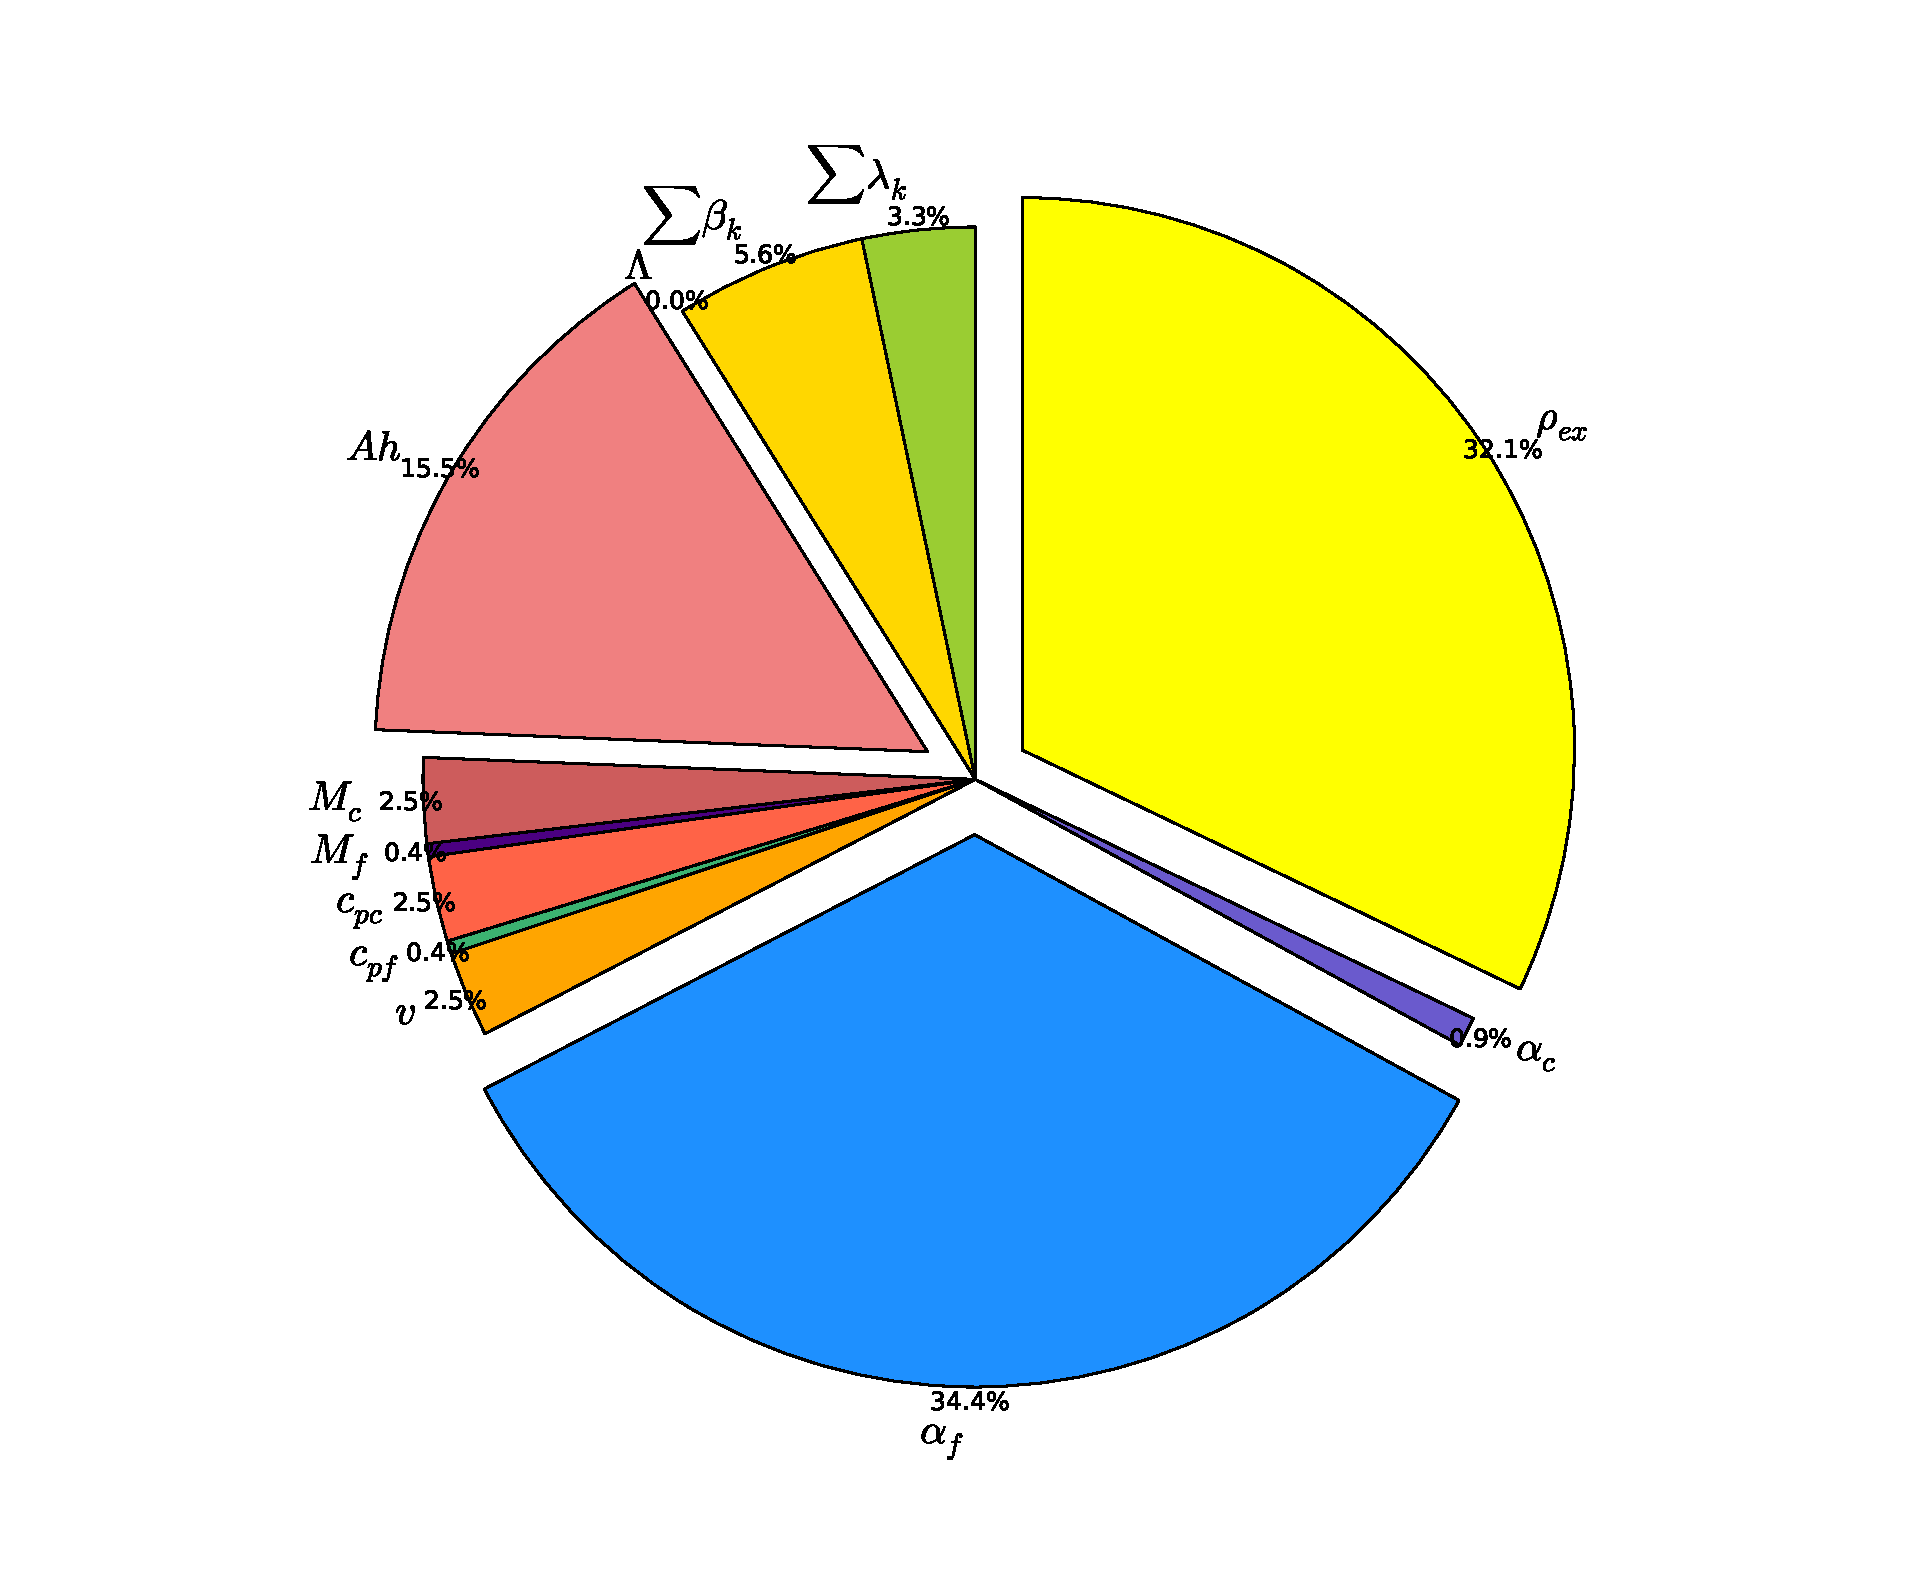
\includegraphics[width=0.6\textwidth]{./pk_importance_pie.pdf}
\end{figure}

\end{frame}
%%%%%%%%%%%%%%%%%%%%%%%%%%%%%%%%%%%%%%%%%%%%%%%%%%%%%%%%%%%%%%%%%%%%%%%%%%%%%%%%%%%%%%%%
\begin{frame}
\frametitle{Morris' Algorithm Sensitivity Analysis}

\begin{itemize}
  \item Algorithm visually identifies $Ah$, $\alpha_d$, and $\rho_{max}$ to be "important variables".
\end{itemize}

\begin{figure}
  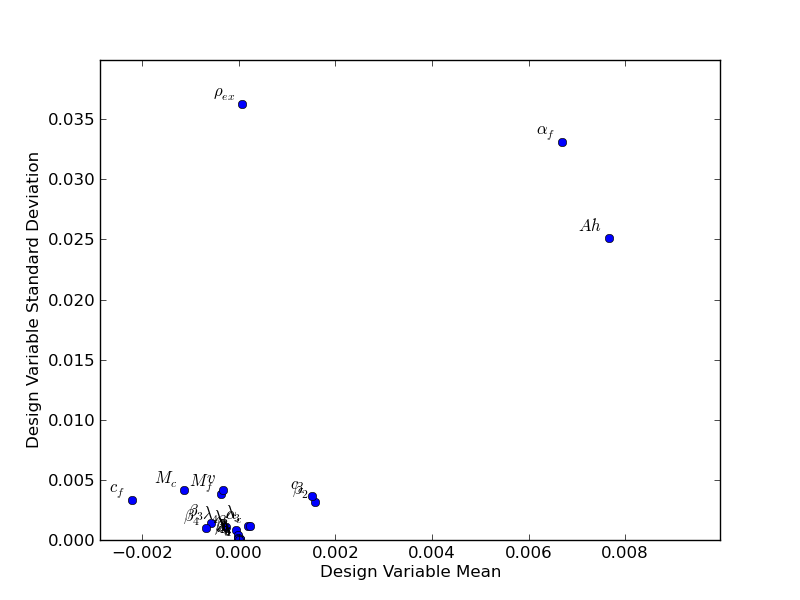
\includegraphics[width=0.75\textwidth]{./importantvariables.png}
\end{figure}

\end{frame}
%%%%%%%%%%%%%%%%%%%%%%%%%%%%%%%%%%%%%%%%%%%%%%%%%%%%%%%%%%%%%%%%%%%%%%%%%%%%%%%%%%%%%%%%
\begin{frame}
\frametitle{Statistics from anchored-ANOVA Collocation Surrogate}

\begin{itemize}
  \item Basic statistics for the maximum fuel temperature attained during transient.
  \item A total of 1000 Monte Carlo samples were used to get the statistics for each method (using the same random numbers). 
  \item A Kriging surrogate based on 3 "important variables" was constructed and also sampled 1000 times for a mean normalized temperature of $1.03198 \pm 0.002299$. 
\end{itemize}

\begin{table}[h] 
\centering
\resizebox{\textwidth}{!}{%
\begin{tabular}{||c|c|c|c|c||} 
\hline \hline
\textbf{Method} & \textbf{Mean} & \textbf{99\% CI} & \textbf{Standard Dev.} & \textbf{99\% CI} \\ \hline
1D ANOVA CC  & 1.03193 & (1.03175, 1.03211) & 0.002187 & (0.002068, 0.002320) \\ \hline
All ANOVA CC & 1.03193 & (1.03175, 1.03211) & 0.002196 & (0.002076, 0.002330) \\ \hline
1D ANOVA GP  & 1.03193 & (1.03175, 1.03211) & 0.002187 & (0.002068, 0.002320) \\ \hline
All ANOVA GP & 1.03193 & (1.03175, 1.03211) & 0.002196 & (0.002076, 0.002330) \\ \hline
True Function & 1.03193 & (1.03175, 1.03211) & 0.002196 & (0.002076, 0.002330) \\ 
\hline \hline
\end{tabular}}
\end{table}

\end{frame}
%%%%%%%%%%%%%%%%%%%%%%%%%%%%%%%%%%%%%%%%%%%%%%%%%%%%%%%%%%%%%%%%%%%%%%%%%%%%%%%%%%%%%%%%
\begin{frame}
\frametitle{Statistics from anchored-ANOVA Collocation Surrogate}

\begin{figure}
  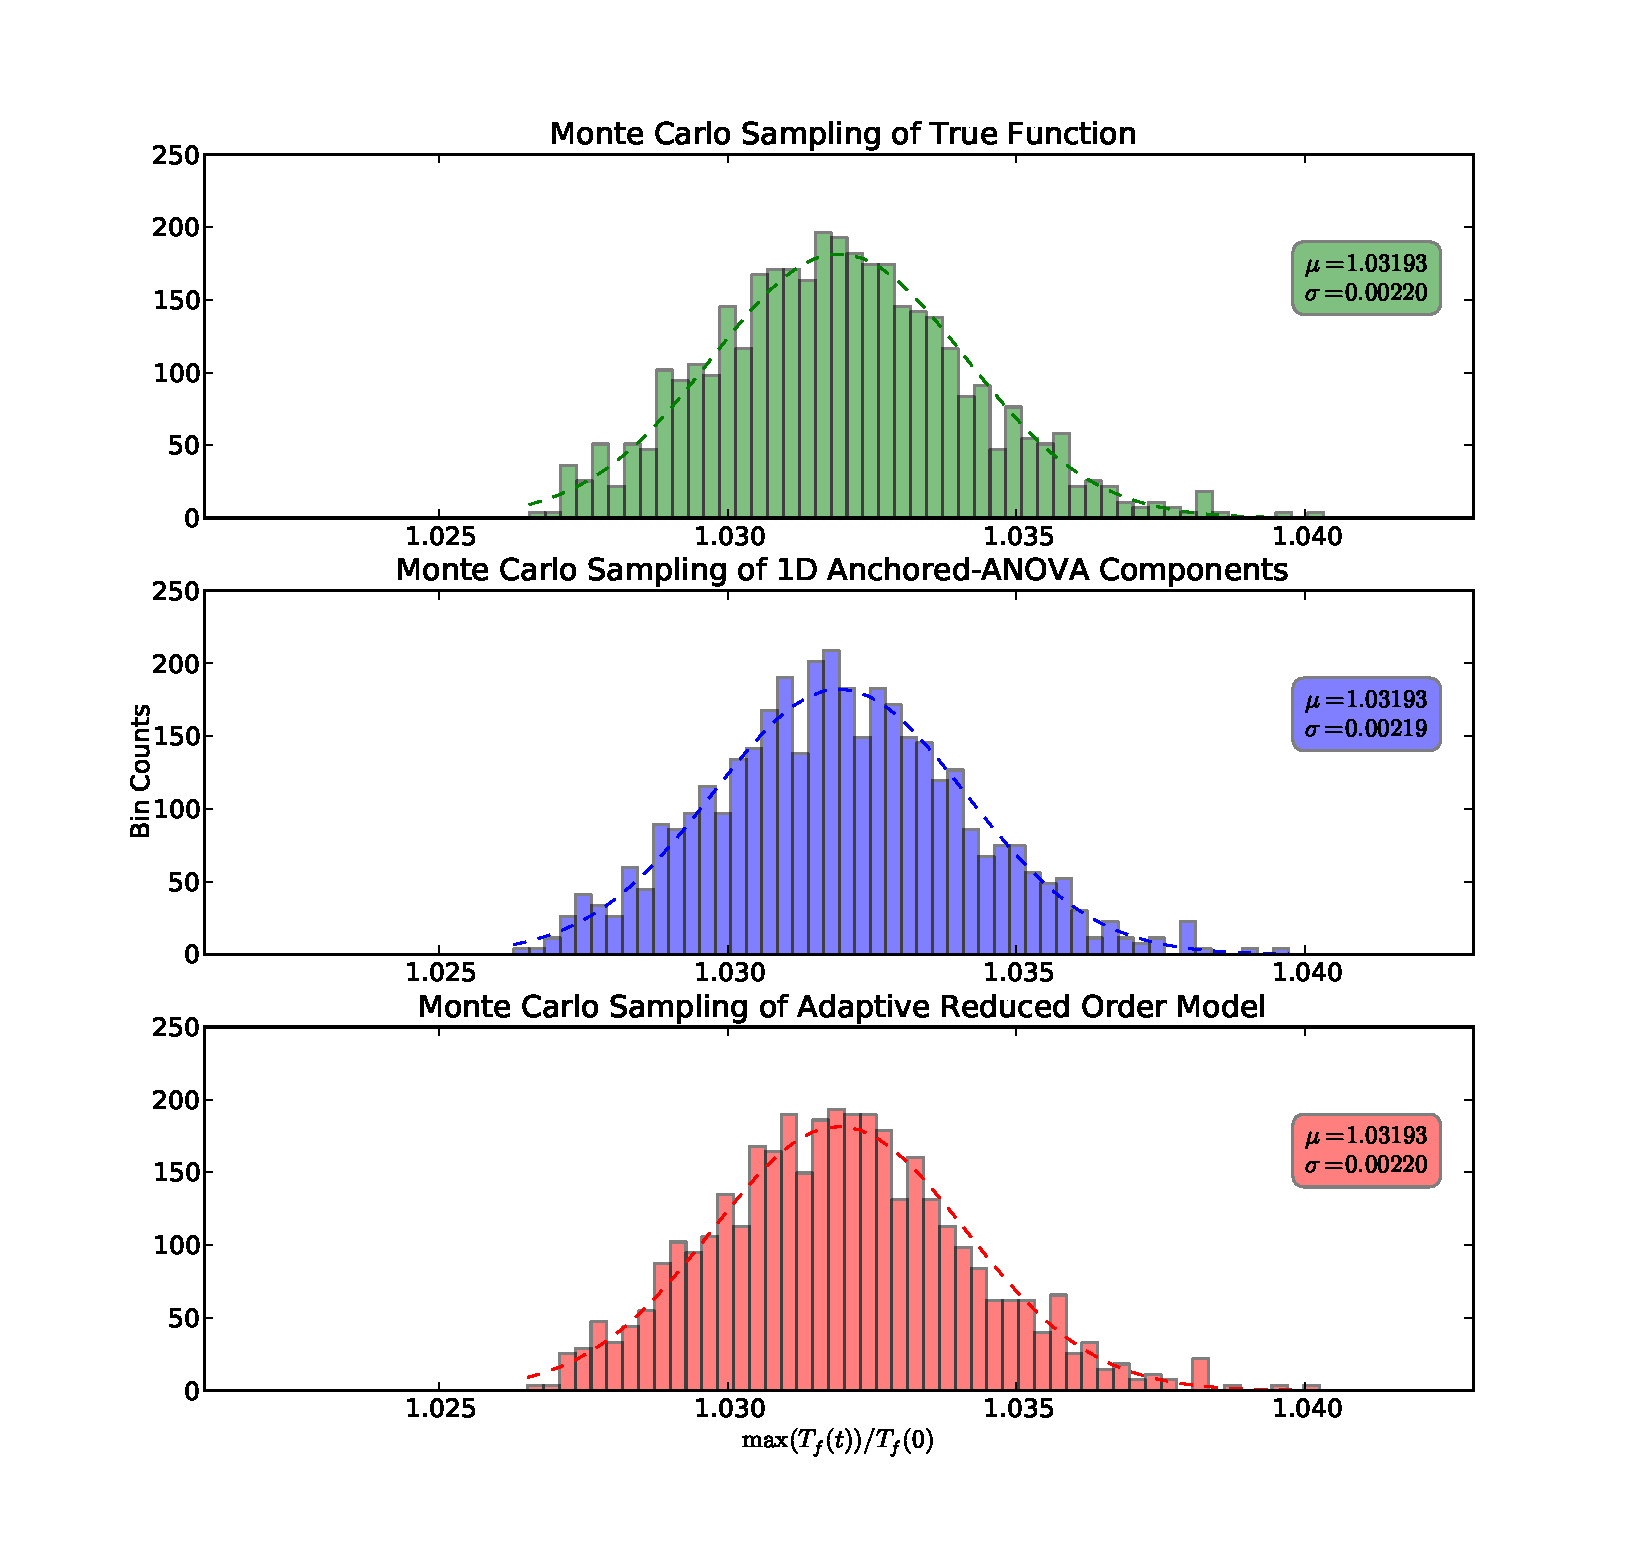
\includegraphics[width=.63\textwidth]{./pk_histograms.pdf}
\end{figure}

\end{frame}
%%%%%%%%%%%%%%%%%%%%%%%%%%%%%%%%%%%%%%%%%%%%%%%%%%%%%%%%%%%%%%%%%%%%%%%%%%%%%%%%%%%%%%%%
\begin{frame}
\frametitle{Statistics from anchored-ANOVA Collocation Surrogate}

\begin{itemize}
  \item Higher-order ANOVA components built only to model interaction effects between $Ah$, $\alpha_d$, and $\rho_{max}$. 
  \item Surrogate consisting entirely of first-order components required 126 function evaluations. 
\end{itemize}

\begin{figure}
  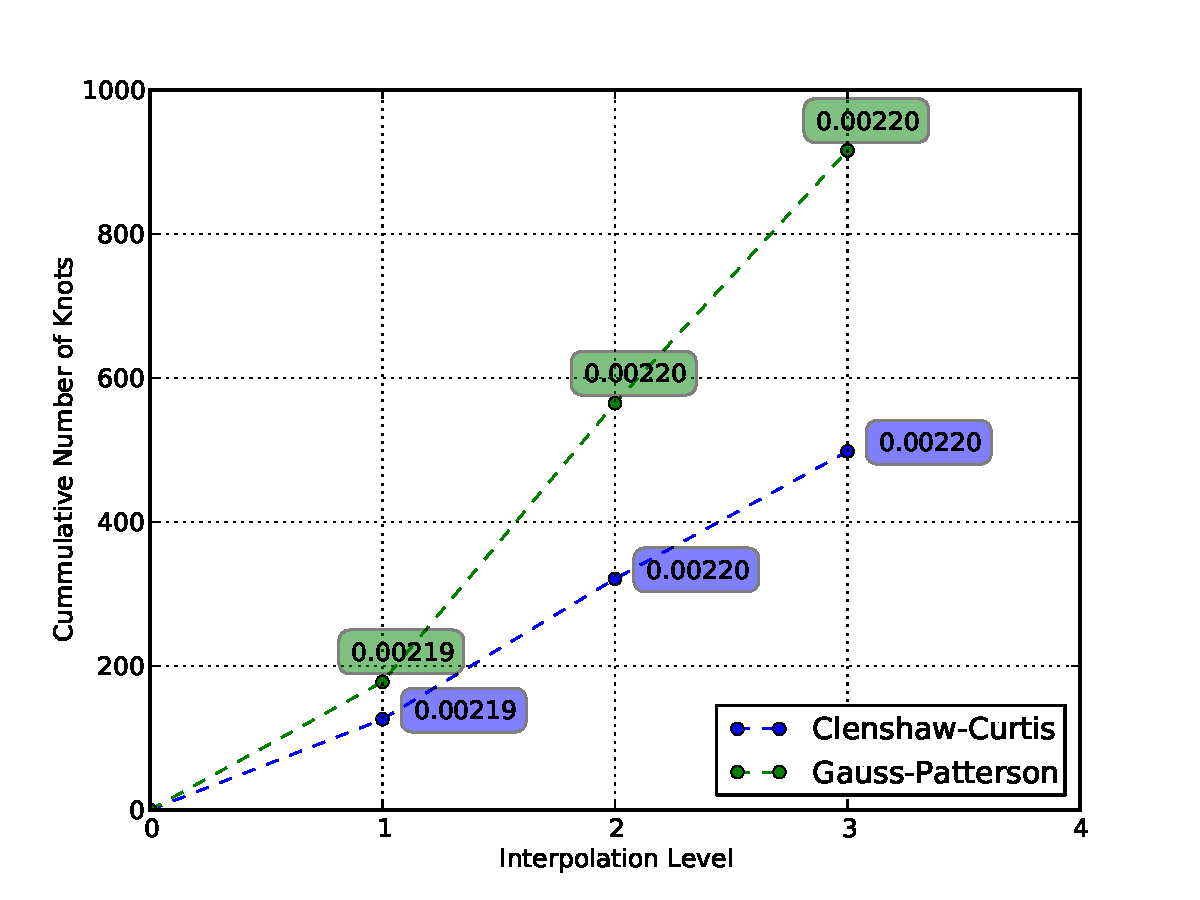
\includegraphics[width=.63\textwidth]{./pk_sparse_grid_numknots.pdf}
\end{figure}

\end{frame}
%%%%%%%%%%%%%%%%%%%%%%%%%%%%%%%%%%%%%%%%%%%%%%%%%%%%%%%%%%%%%%%%%%%%%%%%%%%%%%%%%%%%%%%%
\begin{frame}
\frametitle{Calculating Sensitivity Coefficients on anchored-ANOVA Collocation Surrogates}

\begin{table}[h] 
\centering
\resizebox{\textwidth}{!}{%
\begin{tabular}{||c|c|c|c||} 
\hline \hline
\textbf{Random Variable} & \textbf{1D ANOVA CC} & \textbf{All ANOVA CC} & \textbf{Central Diff.} \\ \hline
$\lambda_4$  &  9.7308E-04 &  9.7309E-04 &  9.7379E-04 \\ \hline
$\beta_2$    & -2.6582E-03 & -2.6582E-03 & -2.6616E-03 \\ \hline
$\Lambda$    & -8.9294E-08 & -8.9295E-08 & -8.9364E-08 \\ \hline
\colorbox{yellow}{$Ah$}         &  1.2553E-02 &  1.2553E-02 &  1.2584E-02 \\ \hline
$M_c$        &  1.8753E-03 &  1.8753E-03 &  1.8716E-03 \\ \hline
$M_f$        & -3.6695E-04 & -3.6695E-04 & -3.6360E-04 \\ \hline
$c_{pc}$     &  1.8753E-03 &  1.8753E-03 &  1.8903E-03 \\ \hline
$c_{pf}$     & -3.6695E-04 & -3.6695E-04 & -3.5976E-04 \\ \hline
$v$          &  1.8838E-03 &  1.8839E-03 &  1.9177E-03 \\ \hline
\colorbox{yellow}{$\alpha_d$}  & -2.6655E-02 & -2.6656E-02 & -2.6625E-02 \\ \hline
$\alpha_c$   &  8.4387E-04 &  8.4387E-04 &  8.7194E-04 \\ \hline
\colorbox{yellow}{$\rho_{max}$} &  3.1164E-02 &  3.1164E-02 &  3.1272E-02 \\ 
\hline \hline
\end{tabular}}
\end{table}

\end{frame}
%%%%%%%%%%%%%%%%%%%%%%%%%%%%%%%%%%%%%%%%%%%%%%%%%%%%%%%%%%%%%%%%%%%%%%%%%%%%%%%%%%%%%%%%
\subsection{TMI Minicore}

\begin{frame}
\frametitle{Three Mile Island (TMI) Minicore Problem Statement}

\begin{itemize}
  \item Build surrogate for TMI Minicore power distribution using core simulator code PARCS.
  \item Total of 25 homogenized, two-group cross sections are used as design variables.  
\end{itemize}

\begin{figure}
  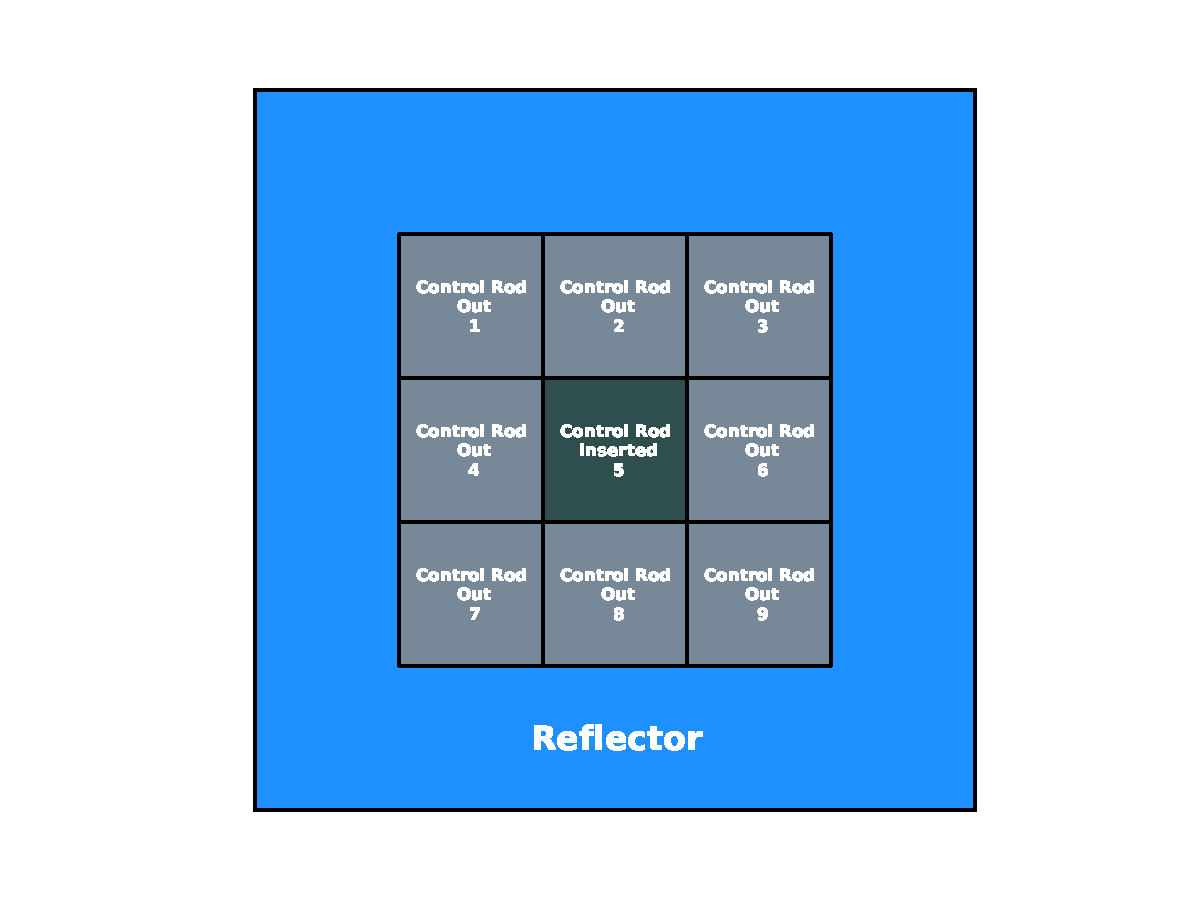
\includegraphics[width=.6\textwidth]{./tmi_minicore.pdf}
\end{figure} 

\end{frame}
%%%%%%%%%%%%%%%%%%%%%%%%%%%%%%%%%%%%%%%%%%%%%%%%%%%%%%%%%%%%%%%%%%%%%%%%%%%%%%%%%%%%%%%%
\begin{frame}
\frametitle{TMI Minicore Problem Data}

\begin{itemize}
  \item The few group, homogenized cross section description for each fuel assembly consists of transport, absorption, nu-fission, and scatter cross sections along with values for ADFs. 
  \item For a two-group problem the total number of cross sections to describe an assembly is nine. 
  \item Since the homogenized reflector region does not support fission only seven homogenized cross sections are required to describe it.
  \item Few-group covariance matrix is obtained using the 'Two-Step' method based on a total of 300 transport calculations with perturbed multigroup cross sections. 
\end{itemize}

\end{frame}
%%%%%%%%%%%%%%%%%%%%%%%%%%%%%%%%%%%%%%%%%%%%%%%%%%%%%%%%%%%%%%%%%%%%%%%%%%%%%%%%%%%%%%%%
\begin{frame}
\frametitle{Morris' Algorithm Sensitivity Study}

\begin{figure}
  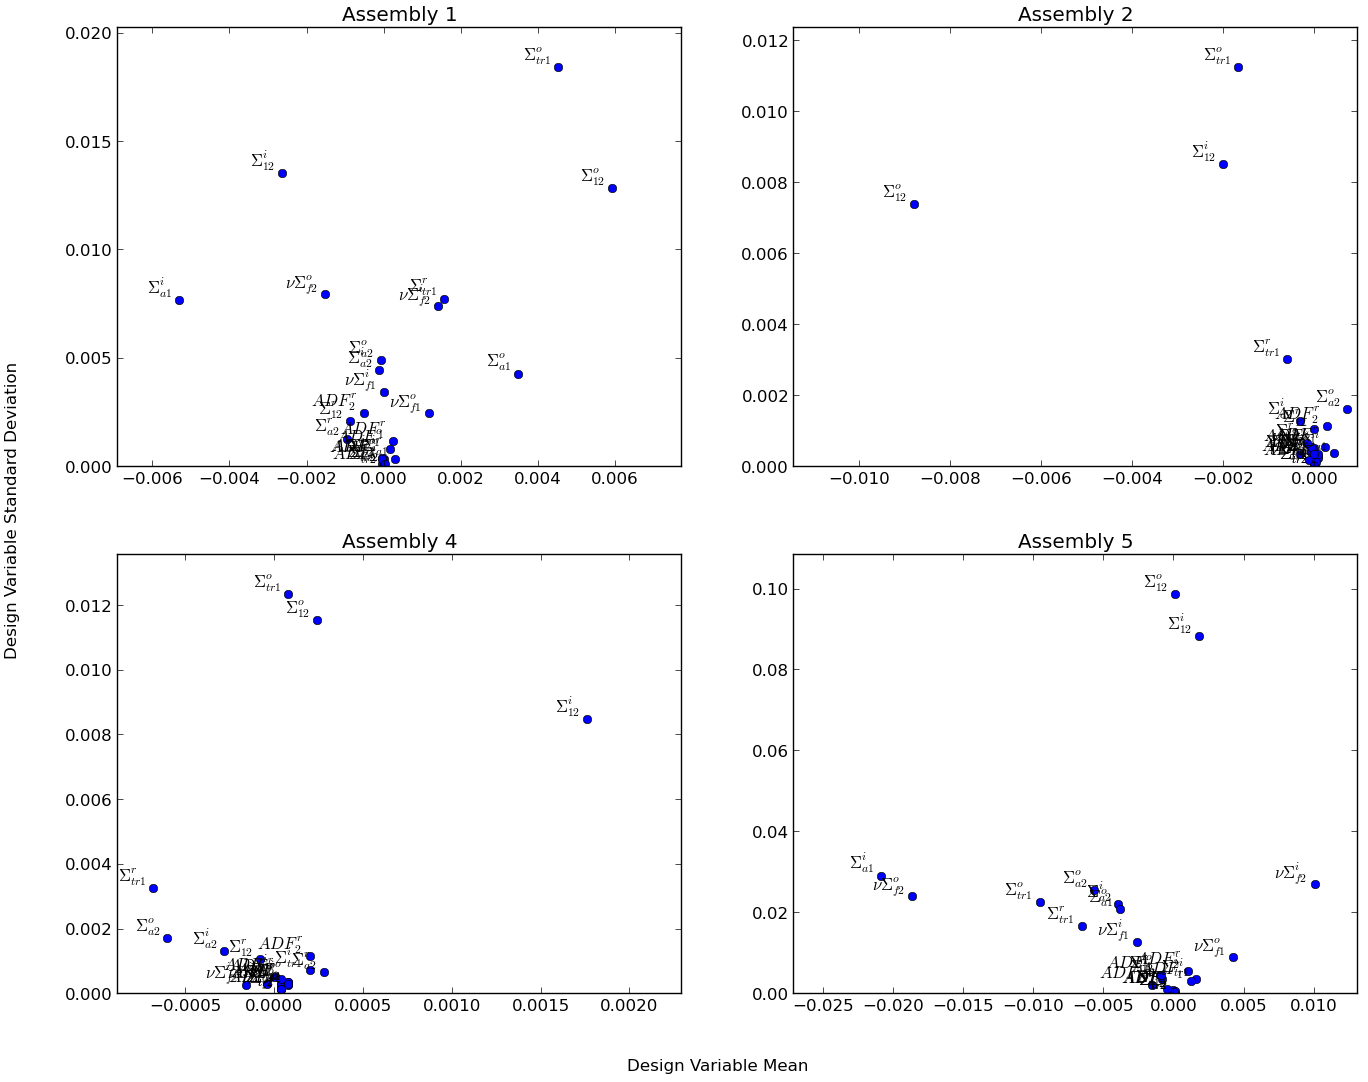
\includegraphics[width=0.85\textwidth]{./tmi_important_vars.png}
\end{figure} 

\end{frame}
%%%%%%%%%%%%%%%%%%%%%%%%%%%%%%%%%%%%%%%%%%%%%%%%%%%%%%%%%%%%%%%%%%%%%%%%%%%%%%%%%%%%%%%%
\begin{frame}
\frametitle{Kriging Surrogate}

\begin{itemize}
  \item Kriging surrogate is constructed for the core power as a function of $\Sigma_{a1}^i$, $\nu\Sigma_{f2}^i$, $\Sigma_{12}^i$, $\Sigma_{tr1}^o$, $\nu\Sigma_{f2}^o$ and $\Sigma_{12}^o$. 
  \item Using these variables a sampling plan consisting of 20 true PARCS evaluations was designed.
  \item Based on the optimized sampling plan a Kriging surrogate was constructed and sampled 500 times in accordance with the six design variables' covariance matrix.
\end{itemize}

\end{frame}
%%%%%%%%%%%%%%%%%%%%%%%%%%%%%%%%%%%%%%%%%%%%%%%%%%%%%%%%%%%%%%%%%%%%%%%%%%%%%%%%%%%%%%%%
\begin{frame}
\frametitle{Sampling the Kriging Surrogate}

\begin{columns}
 \begin{column}{0.5\textwidth}
  \centering
  Kriging Surrogate Statistics
  \begin{table}
  \resizebox{\textwidth}{!}{%
   \begin{tabular}{||c|c|c|c||} 
    \hline \hline
    \textbf{Assembly} & \textbf{Mean} & \textbf{99\% CI} & \textbf{Standard Dev.} \\ \hline
     1 & 0.8385 & (0.8384, 0.8386) & 0.0010\\ \hline 
    2 & 1.1499 & (1.1497, 1.1500) & 0.0013  \\ \hline
    3 & 0.8384 & (0.8383, 0.8386) & 0.0010  \\ \hline
    4 & 1.1499 & (1.1497, 1.1500) & 0.0013  \\ \hline
    5 & 1.0465 & (1.0462, 1.0467) & 0.0022  \\ \hline
    6 & 1.1499 & (1.1497, 1.1500) & 0.0013  \\ \hline
    7 & 0.8384 & (0.8383, 0.8386) & 0.0010  \\ \hline
    8 & 1.1499 & (1.1497, 1.1500) & 0.0013  \\ \hline
    9 & 0.8384 & (0.8383, 0.8386) & 0.0010  \\
    \hline \hline
   \end{tabular}}
  \end{table}
 \end{column}
 \begin{column}{0.5\textwidth}
  \centering
  PARCS Two-Step Statistics
  \begin{table}
   \resizebox{\textwidth}{!}{%
    \begin{tabular}{||c|c|c|c||} 
     \hline \hline
     \textbf{Assembly} & \textbf{Mean} & \textbf{99\% CI} & \textbf{Standard Dev.} \\ \hline
     1 & 0.8387 & (0.8386, 0.8388) & 0.0007 \\ \hline 
     2 & 1.1499 & (1.1498, 1.1500) & 0.0011  \\ \hline
     3 & 0.8387 & (0.8386, 0.8388) & 0.0007  \\ \hline
     4 & 1.1499 & (1.1498, 1.1500) & 0.0011  \\ \hline
     5 & 1.0453 & (1.0450, 1.0456) & 0.0027 \\ \hline
     6 & 1.1499 & (1.1498, 1.1500) & 0.0011  \\ \hline
     7 & 0.8387 & (0.8386, 0.8388) & 0.0007  \\ \hline
     8 & 1.1499 & (1.1498, 1.1500) & 0.0011  \\ \hline
     9 & 0.8387 & (0.8386, 0.8388) & 0.0007  \\ 
    \hline \hline
   \end{tabular}}
  \end{table} 
 \end{column}
\end{columns}

\end{frame}
%%%%%%%%%%%%%%%%%%%%%%%%%%%%%%%%%%%%%%%%%%%%%%%%%%%%%%%%%%%%%%%%%%%%%%%%%%%%%%%%%%%%%%%%
\begin{frame}
\frametitle{anchored-ANOVA Collocation Surrogate}

\begin{itemize}
  \item Constructed surrogate using only first-order components.
  \item Required 123 evaluations of PARCS using Clenshaw-Curtis abscissas.
  \item Hierarchical surplus of $10^{-4}$ used to designate convergence.
  \item Surrogate sampled 500 times and multivariate distributions between assembly boxes calculated and compared to "true" solution. 
\end{itemize}

\end{frame}
%%%%%%%%%%%%%%%%%%%%%%%%%%%%%%%%%%%%%%%%%%%%%%%%%%%%%%%%%%%%%%%%%%%%%%%%%%%%%%%%%%%%%%%%
\begin{frame}
\frametitle{Using anchored-ANOVA Collocation Surrogate to Reproduce Multivariate Distribution}

\begin{figure}
 \begin{center}
  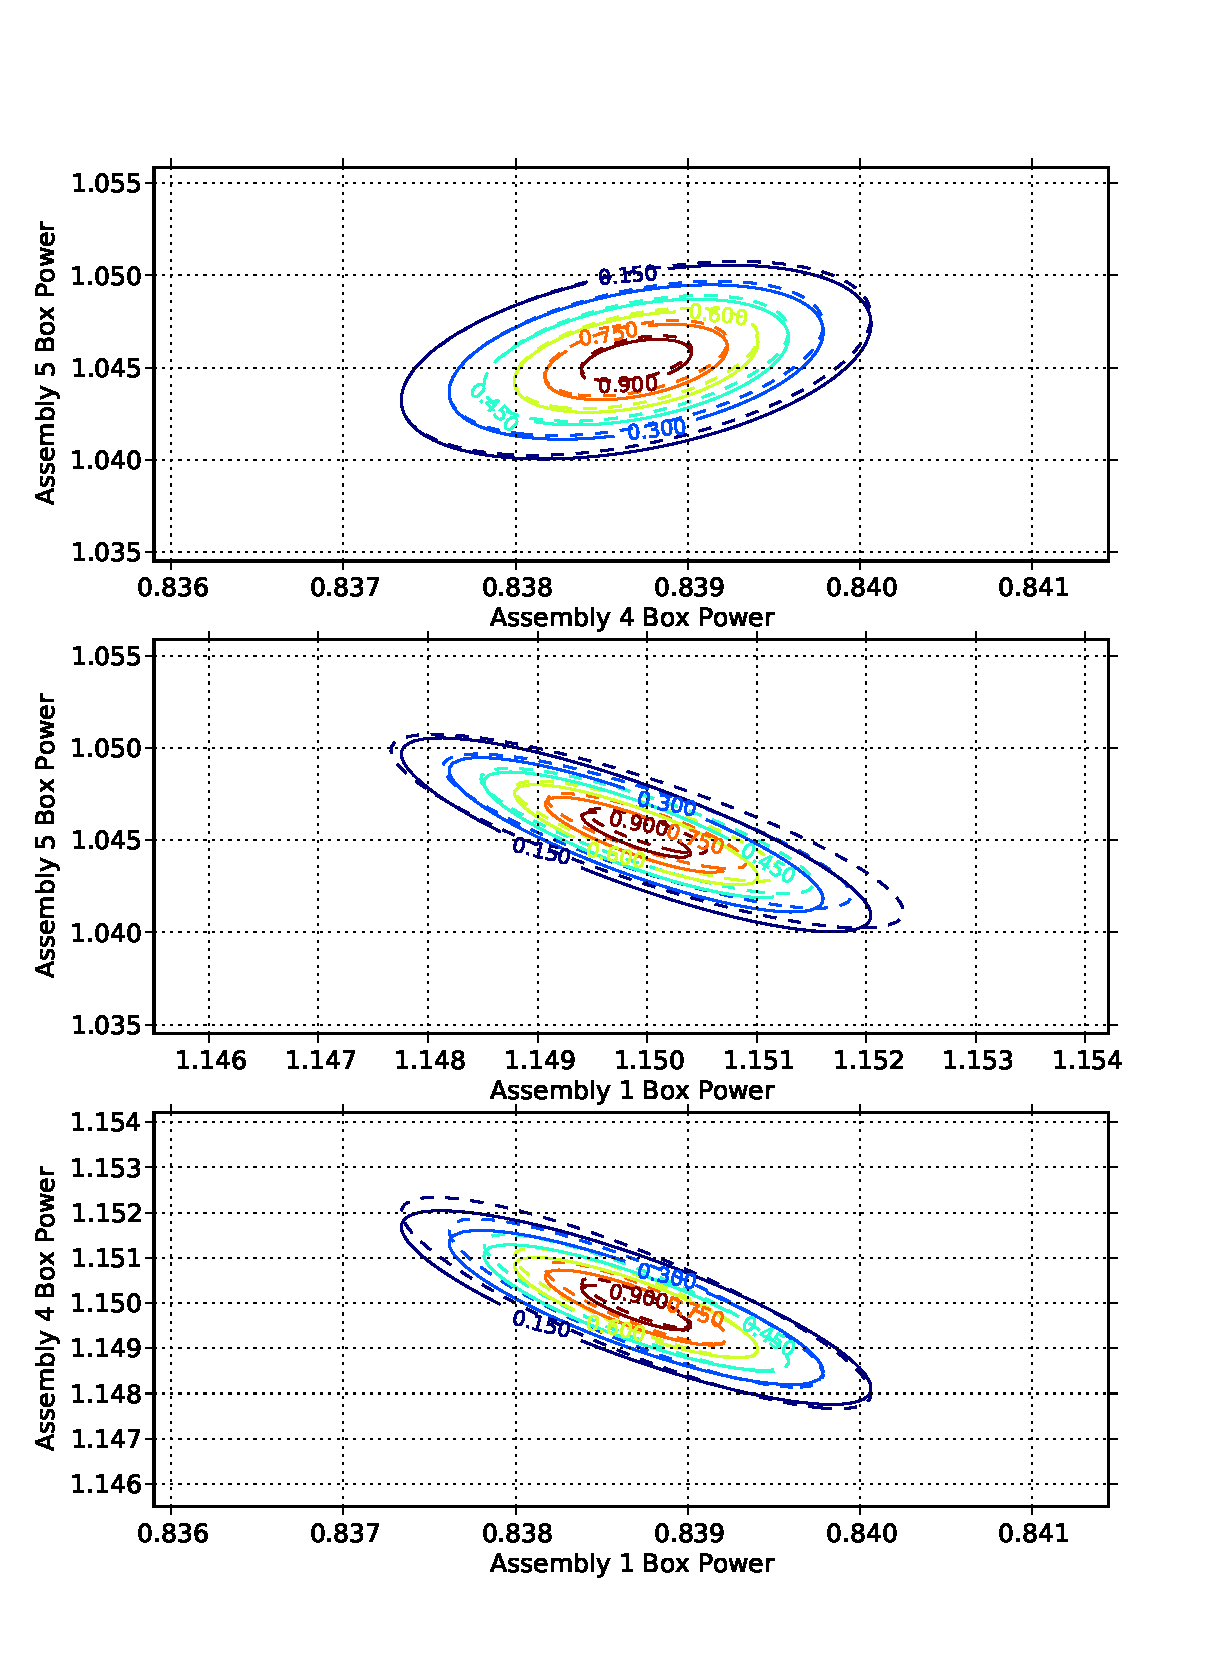
\includegraphics[width=0.50\textwidth]{./tmi_correlations.pdf}
 \end{center}
\end{figure} 

\end{frame}
%%%%%%%%%%%%%%%%%%%%%%%%%%%%%%%%%%%%%%%%%%%%%%%%%%%%%%%%%%%%%%%%%%%%%%%%%%%%%%%%%%%%%%%%

% CLOSING REMARKS
\section{Closing Remarks}

%%%%%%%%%%%%%%%%%%%%%%%%%%%%%%%%%%%%%%%%%%%%%%%%%%%%%%%%%%%%%%%%%%%%%%%%%%%%%%%%%%%%%%%%
\begin{frame}
\frametitle{Original Contributions of Research}

\begin{itemize}
  \item Surrogate use to replace expensive nuclear fuel performance simulations for calibration, optimization and inference.
  \item Folding in fuel performance experimental data with surrogate simulations to improve predictive capabilities of fuel performance codes.  
  \item Use of the anchored-ANOVA decomposition coupled with collocation in nuclear engineering applications.
  \item Application of surrogate methods to multiphysics code systems. 
  \item Use of dimension reduction techniques along with Kriging never before applied to nuclear fuel performance modeling.   
\end{itemize}

\end{frame}
%%%%%%%%%%%%%%%%%%%%%%%%%%%%%%%%%%%%%%%%%%%%%%%%%%%%%%%%%%%%%%%%%%%%%%%%%%%%%%%%%%%%%%%%
\begin{frame}
\frametitle{Work Left to be Completed}

\begin{itemize}
  \item Apply methods described here to construct surrogate for Ris\o~AN3 fission gas release model in BISON using DAKOTA framework.
  \item Use surrogate to infer "true" value of fission gas release parameters by folding in  data from power ramp experiment.
  \item Replace BISON with coupled BISON/MPACT and repeat to study effects building a surrogate on a multiphysics code system.        
\end{itemize}

\end{frame}
%%%%%%%%%%%%%%%%%%%%%%%%%%%%%%%%%%%%%%%%%%%%%%%%%%%%%%%%%%%%%%%%%%%%%%%%%%%%%%%%%%%%%%%%
\begin{frame}
\frametitle{The End}

\centering
Thank you

\end{frame}
%%%%%%%%%%%%%%%%%%%%%%%%%%%%%%%%%%%%%%%%%%%%%%%%%%%%%%%%%%%%%%%%%%%%%%%%%%%%%%%%%%%%%%%%

% EXTRAS
\section{Extras}

%%%%%%%%%%%%%%%%%%%%%%%%%%%%%%%%%%%%%%%%%%%%%%%%%%%%%%%%%%%%%%%%%%%%%%%%%%%%%%%%%%%%%%%%
\begin{frame}
\frametitle{Sparse Grid Mechanics Example}

\begin{itemize}
  \item Consider a function of two dimensions $f(x_1, x_2)$, $d=2$. 
  \item Let's calculate the Level 1 (q=3) Smolyak sparse grid interpolant for $f$, $A_{3,2}(f)$.
\end{itemize}

\begin{align*}
A_{3,2}(f) &= A_{2,2}(f) + \Delta A_{3,2} \\
&= \Delta A_{2,2} + \cancel{A_{1,2}(f)} + \Delta A_{3,2} 
\end{align*}

\begin{itemize}
  \item First let's calculate $\Delta A_{2,2}$. 
\end{itemize}

\begin{align*}
    \Delta A_{2,2} = \sum_{\vert\textbf{i}\vert=2}
     \left(f(x_{j_1}^{i_1},x_{j_2}^{i_2}) - 
      \cancel{A_{1,2}(f)(x_{j_1}^{i_1}, x_{j_2}^{i_2})}\right)\cdot
       \left(a_{j_1}^{i_1}\otimes a_{j_2}^{i_2}\right)
\end{align*}

\end{frame}
%%%%%%%%%%%%%%%%%%%%%%%%%%%%%%%%%%%%%%%%%%%%%%%%%%%%%%%%%%%%%%%%%%%%%%%%%%%%%%%%%%%%%%%%
\begin{frame}
\frametitle{Sparse Grid Mechanics Example}

\begin{itemize}
  \item $\vert\textbf{i}\vert=2 \rightarrow i_1 + i_2 = 2 \rightarrow$ sum over the set of $i$ indices $\lbrace (1, 1)\rbrace$.
  \item Using Clenshaw-Curtis for $i=1$ we have $m_i=1$, namely the origin. 
\begin{align*}
 \Delta A_{2,2} = f\left( x_{1}^{1},x_{1}^{1}\right)a_{1}^{1}a_{1}^{1}
\end{align*}
  \item In this case, $a_1^1 = 1$ and $x_1^1=0$ so $\Delta A_{2,2}$ amounts to evaluating the objective function at the hypercube origin. 
\end{itemize}

\end{frame}
%%%%%%%%%%%%%%%%%%%%%%%%%%%%%%%%%%%%%%%%%%%%%%%%%%%%%%%%%%%%%%%%%%%%%%%%%%%%%%%%%%%%%%%%
\begin{frame}
\frametitle{Sparse Grid Mechanics Example}

\begin{itemize}
  \item Now let's calculate $\Delta A_{3,2}$. 
  \item $\vert\textbf{i}\vert=3 \rightarrow i_1 + i_2 = 3 \rightarrow$ sum over the set of $i$ indices $\lbrace (1, 2), (2, 1) \rbrace$.
  \item Using Clenshaw-Curtis for $i=2$ we have $m_i=3$ so $j\in \lbrace 1,2,3\rbrace$
\end{itemize}

\begin{align*}
 \Delta A_{3,2} &= \sum_{\vert\textbf{i}\vert=3}
  \left(f(x_{j_1}^{i_1},x_{j_2}^{i_2}) - 
  A_{2,2}(f)(x_{j_1}^{i_1}, x_{j_2}^{i_2})\right)\cdot
  \left(a_{j_1}^{i_1}\otimes a_{j_2}^{i_2}\right) \\ 
 &= \sum_{\vert\textbf{i}\vert=3}
  \left(f(x_{j_1}^{i_1},x_{j_2}^{i_2}) - 
  f\left( x_{1}^{1},x_{1}^{1}\right)a_{1}^{1}a_{1}^{1}\right)\cdot
  \left(a_{j_1}^{i_1}\otimes a_{j_2}^{i_2}\right)
\end{align*}

\end{frame}
%%%%%%%%%%%%%%%%%%%%%%%%%%%%%%%%%%%%%%%%%%%%%%%%%%%%%%%%%%%%%%%%%%%%%%%%%%%%%%%%%%%%%%%%
\begin{frame}
\frametitle{Sparse Grid Mechanics Example}

\begin{align*}
 \Delta A_{3,2} &= \left[f(x_{1}^{2},x_{1}^{1}) -
  f\left(x_{1}^{1},x_{1}^{1}\right)a_{1}^{1}a_{1}^{1}\right]a_{1}^{2}a_{1}^{1} \\
  &+ \left[f(x_{2}^{2},x_{1}^{1}) -
  f\left(x_{1}^{1},x_{1}^{1}\right)a_{1}^{1}a_{1}^{1}\right]a_{2}^{2}a_{1}^{1} \\ 
  &+ \left[f(x_{3}^{2},x_{1}^{1}) -
  f\left(x_{1}^{1},x_{1}^{1}\right)a_{1}^{1}a_{1}^{1}\right]a_{3}^{2}a_{1}^{1} \\  
  &+ \left[f(x_{1}^{1},x_{1}^{2}) -
  f\left(x_{1}^{1},x_{1}^{1}\right)a_{1}^{1}a_{1}^{1}\right]a_{1}^{1}a_{1}^{2} \\
  &+ \left[f(x_{1}^{1},x_{2}^{2}) -
  f\left(x_{1}^{1},x_{1}^{1}\right)a_{1}^{1}a_{1}^{1}\right]a_{1}^{1}a_{2}^{2} \\
  &+ \left[f(x_{1}^{1},x_{3}^{2}) -
  f\left(x_{1}^{1},x_{1}^{1}\right)a_{1}^{1}a_{1}^{1}\right]a_{1}^{1}a_{3}^{2} \\  
\end{align*}

\begin{itemize}
  \item Due to the nestedness of Clenshaw-Curtis, points can be reused.
  \item For example, $f(x_1^1, x_1^1) = f(x_1^1, x_2^2) = f(x_2^2, x_1^1)$.
\end{itemize}

\end{frame}
%%%%%%%%%%%%%%%%%%%%%%%%%%%%%%%%%%%%%%%%%%%%%%%%%%%%%%%%%%%%%%%%%%%%%%%%%%%%%%%%%%%%%%%%
\begin{frame}
\frametitle{Sparse Grid Mechanics Example}

\begin{itemize}
  \item Putting everything together, the level 1 Sparse grid interpolant is:
\end{itemize}

\begin{align*}
 A_{3,2}(f) &= \Delta A_{2,2} + \Delta A_{3,2} \\
  &= f\left(x_{1}^{1},x_{1}^{1}\right)a_{1}^{1}a_{1}^{1} \\
  &+ \left[f(x_{1}^{2},x_{1}^{1}) -
  f\left(x_{1}^{1},x_{1}^{1}\right)a_{1}^{1}a_{1}^{1}\right]a_{1}^{2}a_{1}^{1} \\
  &+ \left[f(x_{3}^{2},x_{1}^{1}) -
  f\left(x_{1}^{1},x_{1}^{1}\right)a_{1}^{1}a_{1}^{1}\right]a_{3}^{2}a_{1}^{1} \\  
  &+ \left[f(x_{1}^{1},x_{1}^{2}) -
  f\left(x_{1}^{1},x_{1}^{1}\right)a_{1}^{1}a_{1}^{1}\right]a_{1}^{1}a_{1}^{2} \\
  &+ \left[f(x_{1}^{1},x_{3}^{2}) -
  f\left(x_{1}^{1},x_{1}^{1}\right)a_{1}^{1}a_{1}^{1}\right]a_{1}^{1}a_{3}^{2} \\  
\end{align*}

\end{frame}



\end{document}